\documentclass{report}

\setlength{\textwidth}{150mm}
%\setlength{\textheight}{195mm}
\setlength{\oddsidemargin}{9mm}
%\setlength{\evensidemargin}{28mm}
%\setlength{\topmargin}{-10mm}


\usepackage[utf8]{inputenc}
\usepackage{graphicx}
\graphicspath{ {images/} }
\usepackage{caption}
\usepackage{subcaption}
\usepackage{wrapfig}
\usepackage{listings}
\usepackage[spanish]{babel}
\begin{document}
\begin{titlepage}
\centering

\begin{figure}[t]

\includegraphics[scale=0.5]{images/urjc_logo.png}
\centering
\vspace{0.5cm} %Espacios despúes de la imagen
\end{figure}

{\scshape\Large Escuela Técnica Superior de Ingeniería de Telecomunicación \par}
\vspace{1cm}
{\scshape\Large Grado en Ingeniería en Sistemas de Telecomunicación \par}
\vspace{3cm}
{\bfseries\LARGE INTEGRACIÓN DE ROBOTS FÍSICOS EN LA PLATAFORMA KIBOTICS \par}
\vspace{3cm}
{\itshape\Large Trabajo Fin de Grado \par}
\vfill
{\Large Autor: }
{\Large David ValladaresVigara \par}
{\Large Tutores: }
{\Large Jose María Cañas Plaza y Julio Manuel Vega Pérez \par}
\vfill
{\Large Curso Académico 2019/2020 \par}
\end{titlepage} 

\renewcommand{\abstractname}{\Large Resumen}
\begin{abstract}



\end{abstract}

\setcounter{tocdepth}{3} %Para que aparezcan las subsubsection{}
\renewcommand{\contentsname}{Índice general}
\tableofcontents
\clearpage

\renewcommand{\listfigurename}{Índice de figuras}
\listoffigures

%\renewcommand{\listtablename}{Índice de tablas}
%\listoftables

\renewcommand{\lstlistingname}{Fragmento}
\renewcommand{\lstlistlistingname}{Indice de Fragmentos}
\lstlistoflistings

\renewcommand{\chaptername}{Capítulo}

%###############################################################################
%############# INTRODUCCION ###################################################
%###############################################################################

\chapter{Introducción}

En este capítulo se introducen las aplicaciones de la robótica para el ambiente educativo y las motivaciones que han llevado al desarrollo del Trabajo de Fin de Grado (TFG). Este TFG se ha desarrollado dentro de la plataforma Kibotics para tratar de mejorar la integración sobre robots reales.

\section{Robótica educativa}

La robótica es la ciencia que estudia el diseño y la construcción de máquinas que permiten realizar y facilitar tareas desempeñadas por el ser humano (Quiroga, 2018). Actualmente puede considerarse una de las áreas de las Tecnologías de la Información y Comunicación (TIC) con más auge, pues cada vez es más habitual el uso de robots limpiadores (p. ej. Roomba de iRobot) (Figura 1.1), asistentes virtuales (p. ej. Alexa de Amazon) o el empleo de brazos robóticos en las cadenas de montaje de las industrias. Por ello, resultan muy beneficiosos en el sector industrial y el de servicios (Salamanca, Barrera y Pérez, 2010).
\\
\begin{figure}
  \centering
    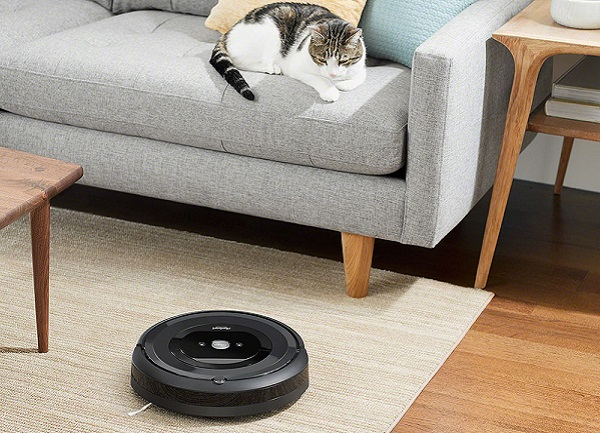
\includegraphics[width=0.4\textwidth]{images/romba.png}
  \caption{Robot aspirador modelo Roomba®}
  \label{Roomba}
\end{figure}
\\

Sin embargo, desde los años sesenta aumentó el interés por introducir la robótica también en el ámbito educativo, creando así la “Robótica educativa” o “Robótica pedagógica”. Se define como una disciplina que permite concebir, diseñar y desarrollar robots educativos para que las personas se puedan iniciar pronto en el mundo de la ciencia y tecnología (Ruiz-Velasco, García y Rosas, 2007). Al combinar diferentes áreas del conocimiento, se ha convertido en una herramienta novedosa que puede utilizarse en las primeras etapas de la educación de los niños y niñas ayudando a potenciar su desarrollo integral (Quiroga, 2018) y que, además, permite que los estudiantes adquieran otras competencias, como la socialización, la creatividad,  la iniciativa y el pensamiento lógico (Bravo y Forero, 2012).
\\

Los orígenes de la robótica educativa se remontan al siglo XX con la teoría constructivista de Jean Piaget, la cual indica que el conocimiento se construye activamente en la mente del estudiante. Esto coincide con la pedagogía del construccionismo de Seymour Papert donde, además, se afirma que lo que construye el individuo debe ser tangible y con un significado personal para él. Algunos desarrollos de la robótica educativa se basan en esta última (González y Jiménez, 2009).
\\

La robótica educativa, por tanto, se considera una herramienta paralela a las asignaturas tradicionales al volverlas más atractivas e integradoras para los estudiantes (Quiroga, 2018). Con ello, ayuda a los alumnos a construir conceptos y a hacer una interpretación personal de la realidad (Salamanca, Barrera y Pérez, 2010).
\\

\subsection{Ejemplo de Metodología para la enseñanza}

Una de las metodologías para llevar a cabo un proceso de trabajo de robótica es la de las cuatro palabras de Báez et al. (2011), representadas en la Figura 1.2. La primera de ellas es “imaginar” porque los estudiantes piensan y debaten sobre dispositivos que pueden ser útiles para resolver un problema o facilitar un trabajo, lo que favorece al pensamiento creativo. A continuación, encontramos la palabra “diseñar”, que les permite crear el artefacto que han imaginado consiguiendo una conexión entre el mundo físico y la imaginación. La tercera es “construir”, que se basa en el montaje de los dispositivos que han diseñado los miembros del grupo de trabajo, por lo que favorece la cooperación y el trabajo manual. La última palabra del proceso es “programar” o dotar de inteligencia a los dispositivos montados a través de un ordenador, mejorando el pensamiento lógico, la autopercepción y el análisis espacial.
\\
\begin{figure}[h!]
  \centering
    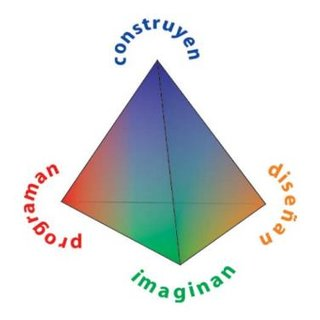
\includegraphics[width=0.4\textwidth]{images/metodologia.png}
  \caption{Las cuatro palabras de la Robótica educativa (Báez et al., 2011).}
  \label{Metodologia}
\end{figure}
\\

\subsection{Aumento de la implantación de la robótica en las aulas}

En la última década, la robótica ha adquirido mucha importancia en un gran número de países (Quiroga, 2018), y cada vez genera más interés implantarla en las aulas (Salamanca, Barrera y Pérez, 2010).
\\

Esto se debe a que aporta muchos beneficios en el proceso de enseñanza-aprendizaje de asignaturas difíciles (Moreno et al., 2012). También es más frecuente la creación de robots para la vida cotidiana, lo que despierta el interés de las personas en ellos (Quiroga, 2018). Además, la existencia de lenguajes de programación orientados a alumnos de menor edad (p. ej. Scratch - Figura 1.3) y la mayor disponibilidad de kits de robótica educativa en el mercado los ha convertido en productos ideales para la iniciación en este campo.
\\
\begin{figure}[h!]
  \centering
    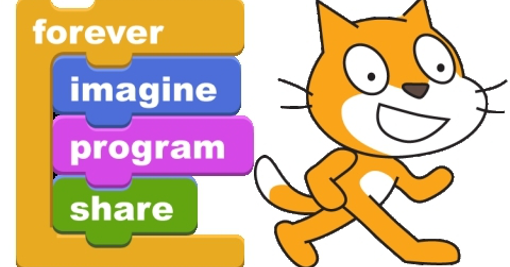
\includegraphics[width=0.3\textwidth]{images/logo_scratch.png}
  \caption{Scratch}
  \label{Scratch}
\end{figure}
\\

Algunos de los robots existentes en el mercado orientados a ese aprendizaje en la robótica son:
\begin{itemize}
	\item \textbf{Mbot}. Diseñado por la empresa MakeBlock y basado en Arduino Uno, una placa electrónica que contiene un microcontrolador programable.
		\begin{figure}[h!]
  			\centering
   			 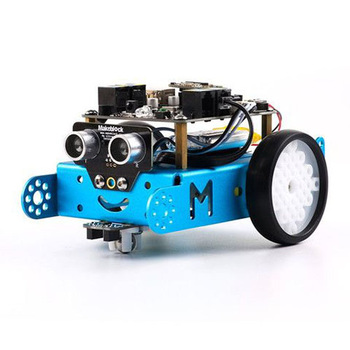
\includegraphics[width=0.3\textwidth]{images/mbot.png}
 			 \caption{Mbot}
 			 \label{Mbot}
		\end{figure}
	\item \textbf{Tello de Ryze Dji }. Es un pequeño dron pensado para que los niños y adultos aprendan su manejo de forma sencilla.
		\begin{figure}[h!]
  			\centering
   			 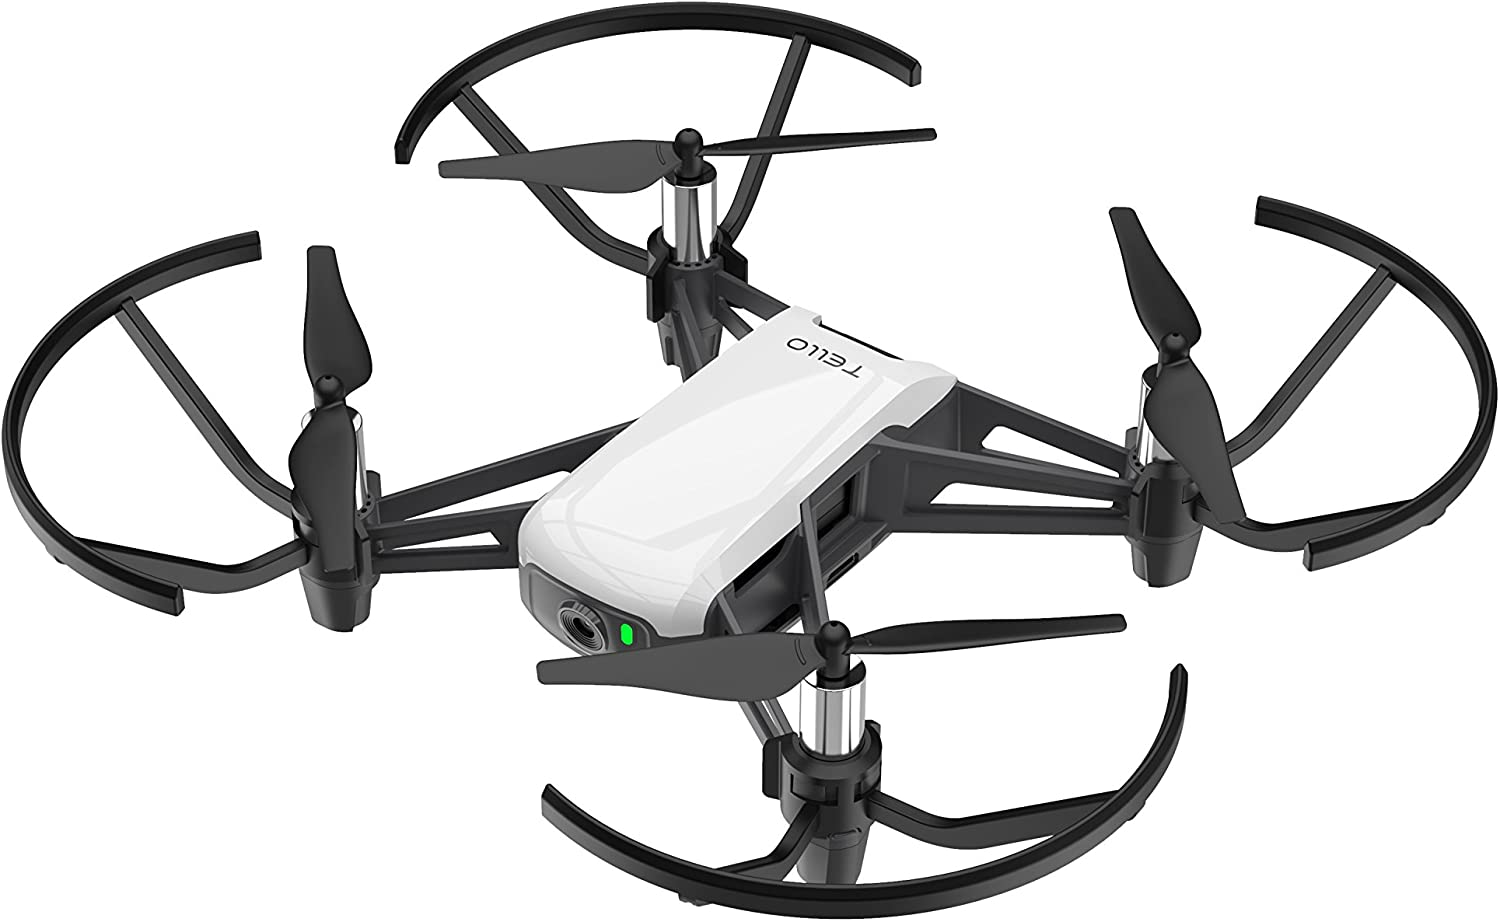
\includegraphics[width=0.3\textwidth]{images/tello.png}
 			 \caption{Tello}
 			 \label{Tello}
		\end{figure}
	\item \textbf{GoPiGo3}. Es un robot con forma de coche creado por Dexter Industries, se caracteriza porque su controladora es una Raspberry Pi 3, un mini-ordenador de bajo conste que le dota de una gran inteligencia.
		\begin{figure}[h!]
  			\centering
   			 \includegraphics[width=0.3\textwidth]{images/GoPiGo.png}
 			 \caption{GoPiGo3}
 			 \label{GoPiGo3}
		\end{figure}
\end{itemize}

Por último, existen aplicaciones y páginas web de programación robótica que facilitan la creación de programas para los robots, como pueden ser Mblock (desarrollada por la empresa MakeBlock y basada en Scratch 3), Bitbloq (creada por la empresa bq, que utiliza bloques para realizar los programas y es compatible con la placa arduino) o Kibotics (llevada a cabo por JdeRobot).
\\

\section{Kibotics}

Kibotics (Figura 1.7) es un entorno web utilizado para la docencia en los campos de robótica, programación y áreas STEM (acrónimo de Science, Technology, Engineering and Mathematics).
\\
\begin{figure}[h!]
  \centering
    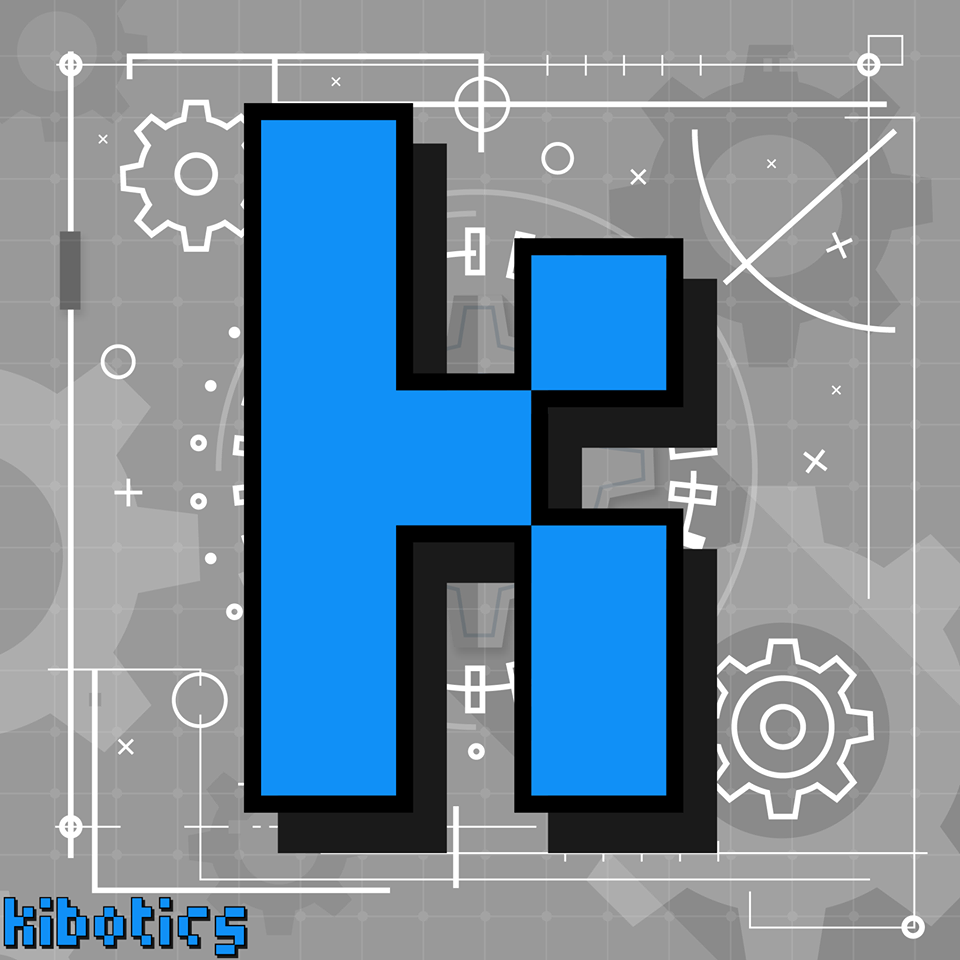
\includegraphics[width=0.3\textwidth]{images/logo_kibotics.png}
  \caption{Logo de Kibotics}
  \label{Logo de Kibotics}
\end{figure}
\\


Ayuda a los alumnos a iniciarse en el mundo de la robótica y la programación de forma sencilla y práctica.
\\

\subsection{Lenguajes soportados en Kibotics}

La plataforma proporciona, actualmente, ejercicios para dos lenguajes de programación. El primero de ellos es Blockly, que fue desarrollado por Google y es muy similar a Scratch. Está orientado para alumnos de menor edad por ser un lenguaje de programación visual basado en una interfaz de bloques que se pueden encajar como si fuera un puzle. Su uso en colegios e institutos es cada vez mayor, ya que está diseñado para que la iniciación al mundo de la programación sea sencilla, divertida y creativa.
\\

Los procedimientos utilizados en la programación de Blockly en Kibotics se clasifican en:
\begin{itemize}
	\item \textit{Serie} : ordenación de los bloques creando una secuencia lógica.

	\item \textit{Bucles}: proporcionan la posibilidad de introducir repeticiones sobre una secuencia deseada.
		
	\item \textit{Variables}: aquellas estructuras de datos en las que se pueden almacenar información a lo largo de la ejecución de un programa.
	
	\item \textit{Operadores lógicos}: devuelve un resultado de verdadero o falso en función de si se cumple o no una determinada condición.
	
	\item \textit{Bloques condicionales}: permiten decidir qué camino lógico tomar en base a una operación lógica.
	
	\item \textit{Operador matemático}: aquellos bloques que permiten realizar una operación matemática.
	
	\item \textit{Robot Api}: se proporciona una interfaz con los actuadores y sensores disponibles para un determinado robot, facilitando así su programación.
\end{itemize}

El segundo es Python, enfocado para alumnos mayores. Constituye uno de los lenguajes de programación con más popularidad en la actualidad según el Índice de Popularidad de Lenguajes de Programación (PYPL PopularitY of Programming Language index, 2020). Es multiparadigma, multiplataforma, gratuito, posee un tipado dinámico e interpretado, es decir, no necesita que un compilador lo procese. Estas características, además de tener una sintaxis legible, permiten un aprendizaje más sencillo que con otros lenguajes de programación como Blockly (Figura 1.8).
\\
\begin{figure}[h!]
  \centering
    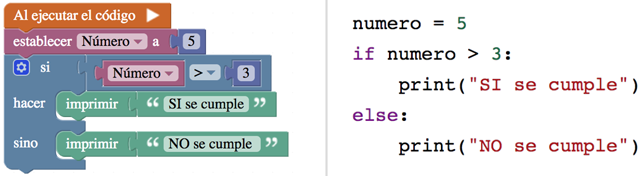
\includegraphics[width=1\textwidth]{images/blockly-vs-python.png}
  \caption{Comparación del mismo código escrito en Blockly (izquierda) y Python (derecha)}
  \label{Comparación del mismo código escrito en Blockly y Python}
\end{figure}
\\

En Kibotics se proporciona una variedad de ejercicios para poner en práctica la programación en Python en diferentes robots. Además, para facilitar el manejo con ellos, se han desarrollado librerías que proporcionan funciones para interactuar con los actuadores y sensores de los robots disponibles. Por ejemplo, en la Figura 1.9 se indican algunas funciones disponibles para el manejo del Dron “Tello”.
\\
\begin{figure}[h!]
  \centering
    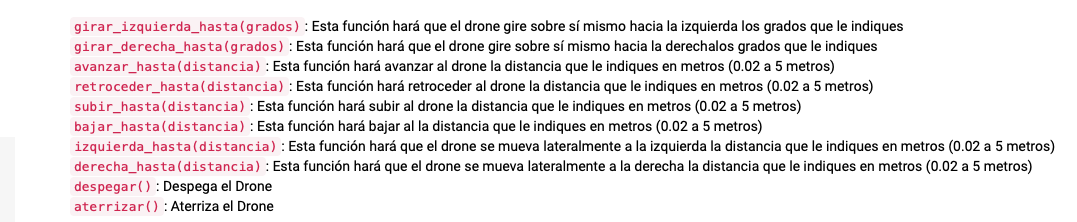
\includegraphics[width=1.1\textwidth]{images/api.png}
  \caption{Funciones disponibles para el Dron “Tello”.}
  \label{Funciones disponibles para el Dron “Tello”.}
\end{figure}
\\

\subsection{Tipos de Robots}

No existe una definición única universal para la palabra “robot”. Por ejemplo, la Real Academia Española (RAE) determina que es una “máquina o ingenio electrónico programable, capaz de manipular objetos y realizar operaciones antes reservadas solo a las personas” (RAE, 2020). También se define como un “sistema compuesto por mecanismos que le permiten hacer movimientos y realizar tareas específicas, programables y eventualmente inteligentes, valiéndose de conceptos de otras áreas del conocimiento” (Salamanca, Barrera y Pérez, 2010).
\\

Un robot se compone, principalmente, de las siguientes partes:
\begin{itemize}
	\item \textit{Esqueleto}. Encargado de soportar los componentes que forman al robot.

	\item \textit{Controladora}. Encargada de procesar los datos obtenidos de los sensores, tomar decisiones y enviar las órdenes a los actuadores.
		
	\item \textit{Sensores o receptores}. Miden magnitudes físicas y las transforman a magnitudes eléctricas. Existen dos tipos, por un lado, están los encargados del entorno que les rodea y, por otro, los del estado interno. Ejemplos de sensores son los infrarrojos, de proximidad, ultrasonido, etc.
	
	\item \textit{Actuadores}. Encargados del movimiento del robot mediante las órdenes recibidas de la controladora.
\end{itemize}

En Kibotics se distinguen dos tipos de robots con los que se puede interactuar: los robots simulados (p. ej. Drone Tello, Mbot, Pibot) y los robots físicos o reales (p. ej. Pibot).
\\

Los robots simulados son robots virtuales que emulan el comportamiento de un robot real, permitiendo al usuario interactuar con él como si fuera uno real (Figura 1.10). Esto se fundamenta en la idea de Robert E. Shannon de simulación como “un proceso de diseñar un modelo de un sistema real y llevar a termino experiencias con él, con la finalidad de comprender el comportamiento del sistema o evaluar nuevas estrategias para el funcionamiento del sistema” (Shannon, 1998).  Al trabajar con ellos, no se necesita su presencia física, se crea una interacción más segura y se puede experimentar con situaciones más complejas o con las que no se posee información.
\\
\begin{figure}[h!]
  \centering
    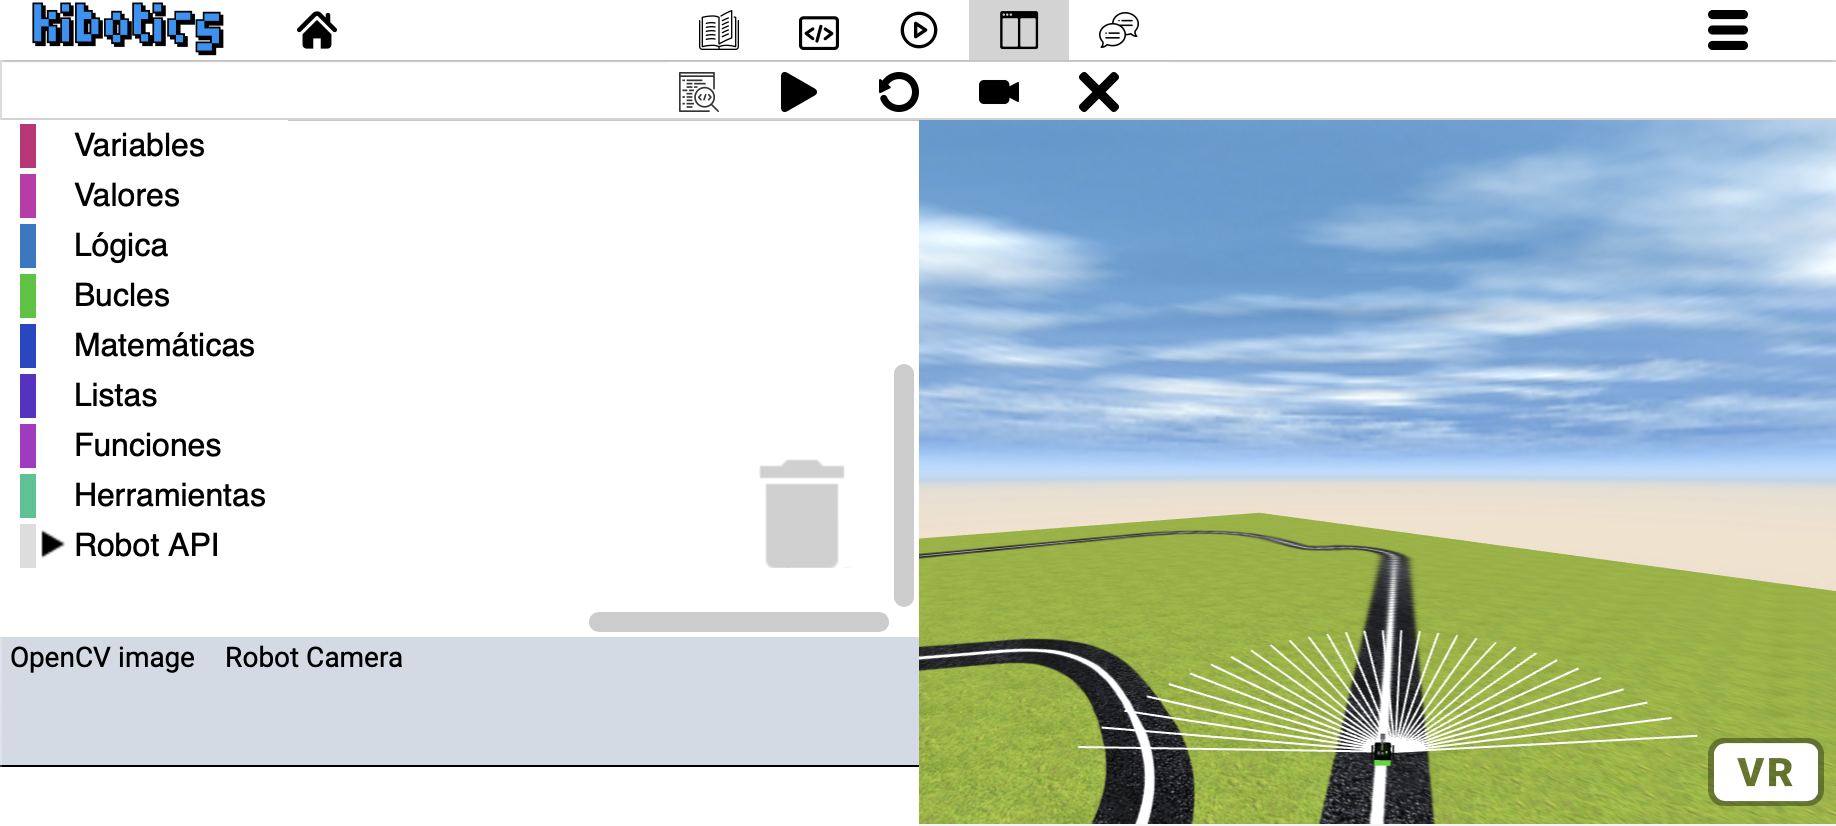
\includegraphics[width=0.9\textwidth]{images/simulado.png}
  \caption{Ejemplo de Robot simulado en Kibotics}
  \label{Ejemplo de Robot simulado en Kibotics}
\end{figure}
\\

En cuanto a los robots físicos o reales, desde Kibotics se da soporte para el desarrollo de programas y envíos sobre algunos de ellos, por ejemplo, para el Pibot mencionado anteriormente. Con ello, se pretende facilitar este proceso de comunicación, que en muchas ocasiones puede no ser sencillo.
\\

En este punto recae la motivación principal para este TFG, que consiste en proporcionar soporte para el uso sobre robots reales, como Mbot, Tello y Gopgio, aunque se hablará más en detalle en el capítulo dos.


%###############################################################################
%############# OBJETIVOS #######################################################
%###############################################################################


\chapter{Objetivos}

Una vez presentado el marco en el que se realiza este TFG, en este capítulo se exponen los objetivos propuestos y los requisitos de este proyecto, además de la metodología de trabajo que se ha llevado a cabo para su resolución.
\section{Objetivos del TFG}

El objetivo principal de este TFG es conseguir integrar nuevos robots reales en la plataforma de Kibotics para poder utilizarlos desde ella, es decir, que desde dicha plataforma seamos capaces de programarlos y de enviarles el programa.
\\
\\
Para la realización del proyecto, se han utilizado tres robots diferentes, cada uno de ellos con una serie de características que les hacen ser interesantes para su integración en esta plataforma. El primero de ellos es el Mbot, que se ha elegido por ser uno de los más populares en el mundo de la Robótica Educativa, ya que tiene un diseño muy atractivo para los niños. Además, está basado en una placa de ArduinoUno, una de las placas más famosas de código abierto y de la que hay mucha documentación y ejemplos de ejercicios disponibles que ayudan en el aprendizaje. El siguiente robot escogido es el Dron Tello debido a que los drones han ganado mucha popularidad en los últimos años y este dron proporciona muy buenas características para aprender sobre este ámbito. Por último, tenemos el GopiGo3 que, al contener una Raspberry Pi, se ha convertido en un robot muy inteligente y flexible. Entre las características que puede ofrecer, por ejemplo, es que se puede conectar una cámara a la Raspberry Pi, lo que le otorga una amplia gama de posibilidades para realizar programas relacionados con la detección de objetos o el análisis de imagen. Por lo tanto, gracias a estos robots los alumnos no solo aprenden temas relacionados con la robótica, sino que también van a introducirse en el mundo de la informática y electrónica.
\\
\\
Hasta ahora, Kibotics incluía algunos robots reales para poder programarlos, entre ellos el ya mencionado Mbot. Sin embargo, este robot solo podía programarse si se utilizaba un ordenador con Linux como sistema operativo. Además, el proceso de envío no era directo, pues cuando el usuario quería enviar el programa realizado al robot, era necesario descargar un ejecutable.
\\
\\
Teniendo esto en cuenta, hemos dividido el objetivo principal en dos objetivos específicos que deben cumplirse en la integración de los robots en la plataforma:
\begin{itemize}
	\item Ser multiplataforma, es decir, se deben poder usar en los principales sistemas operativos (Linux, Windows y MacOs).
	\item El proceso de envío debe ser lo más sencillo posible para evitar que el usuario tenga que hacer instalaciones o configuraciones adicionales. De esta manera conseguimos que las personas con pocos conocimientos en informática también puedan hacer uso de la plataforma.
\end{itemize}
Con ello, se conseguiría estar más cerca del propósito de Kibotics de llevar la robótica al público más general y a los más pequeños.

\section{Metodología}

Durante el desarrollo de este TFG se ha seguido el modelo de diseño iterativo (Figura 2.1), muy utilizado en el desarrollo de software. Se basa en la idea de entregar al cliente algo tangible cuanto antes para que pueda validarlo y, si es necesario, puedan hacerse los cambios de manera rápida sin tener que modificar todo el proyecto por completo. Además, también se deben hacer pequeñas iteraciones para evaluar las funcionalidades en los siguientes ciclos. Este diseño es una buena opción porque aporta cierta flexibilidad, algo muy útil en los procesos de desarrollo del software, los cuales suelen experimentar cambios frecuentes.
\\
\begin{figure}[h!]
  \centering
    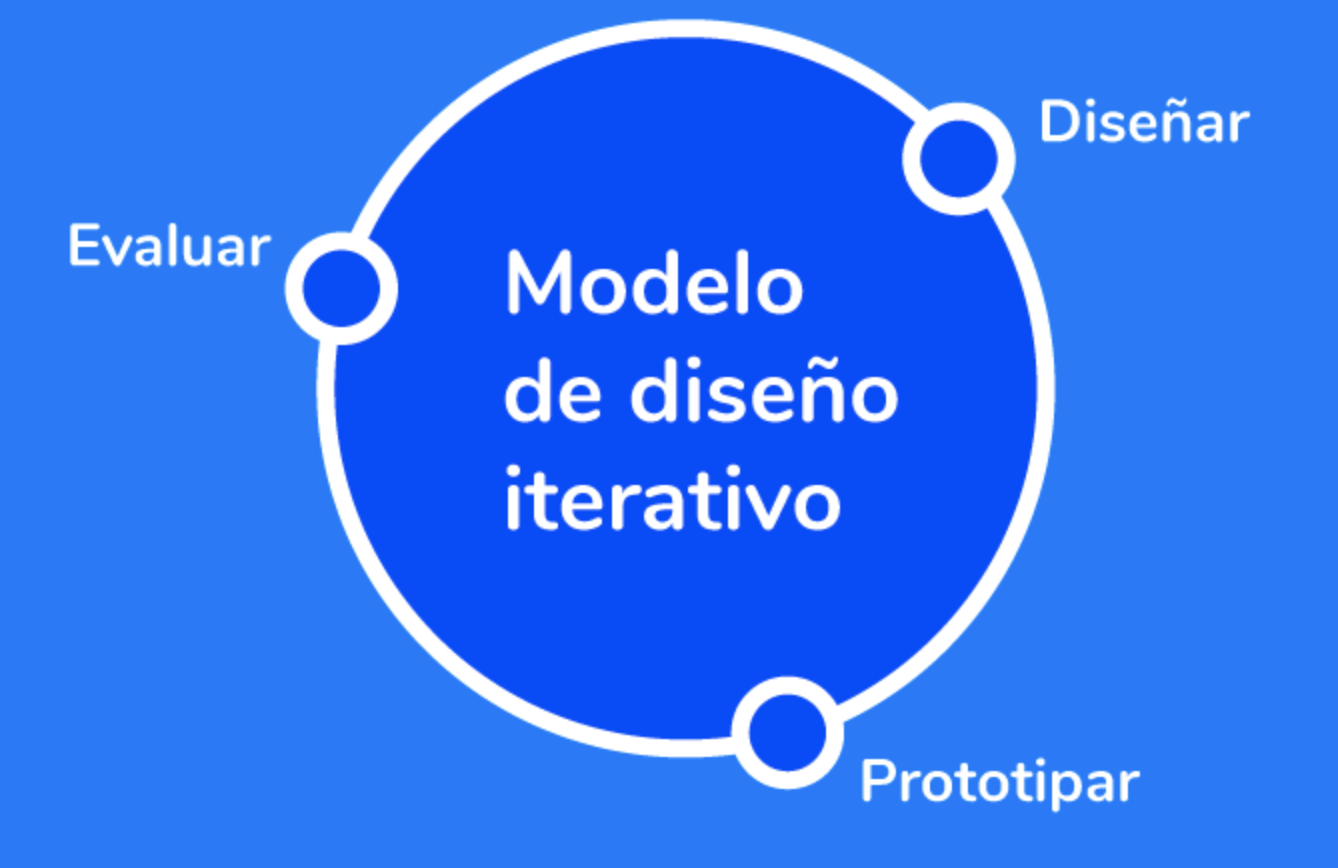
\includegraphics[width=0.5\textwidth]{images/metodologia_interativa.png}
  \caption{Modelo iterativo}
  \label{Modelo iterativo}
\end{figure}
\\
Las ventajas que ofrece esta metodología es que el cliente no tiene que esperar mucho tiempo hasta ver resultados en su proyecto, de manera que puede hacer llegar rápido a la empresa sus opiniones y así tener solventadas las necesidades, tanto del propio cliente como del mercado. Por otro lado, al hacer varias iteraciones, el riesgo ante un problema es pequeño y fácil de solucionar. Todo esto hace que el conocimiento sobre el producto es progresivo y creciente.
\\
\\
Para el seguimiento de este trabajo, se ha utilizado la herramienta de control de versión Git y GitHub. Además, se planificaban reuniones semanales con los tutores del TFG y se creó un blog (Valladares, 2019) donde se registraban las tareas realizadas a lo largo de la semana (Figura 2.2).
\\
\begin{figure}[h!]
  \centering
    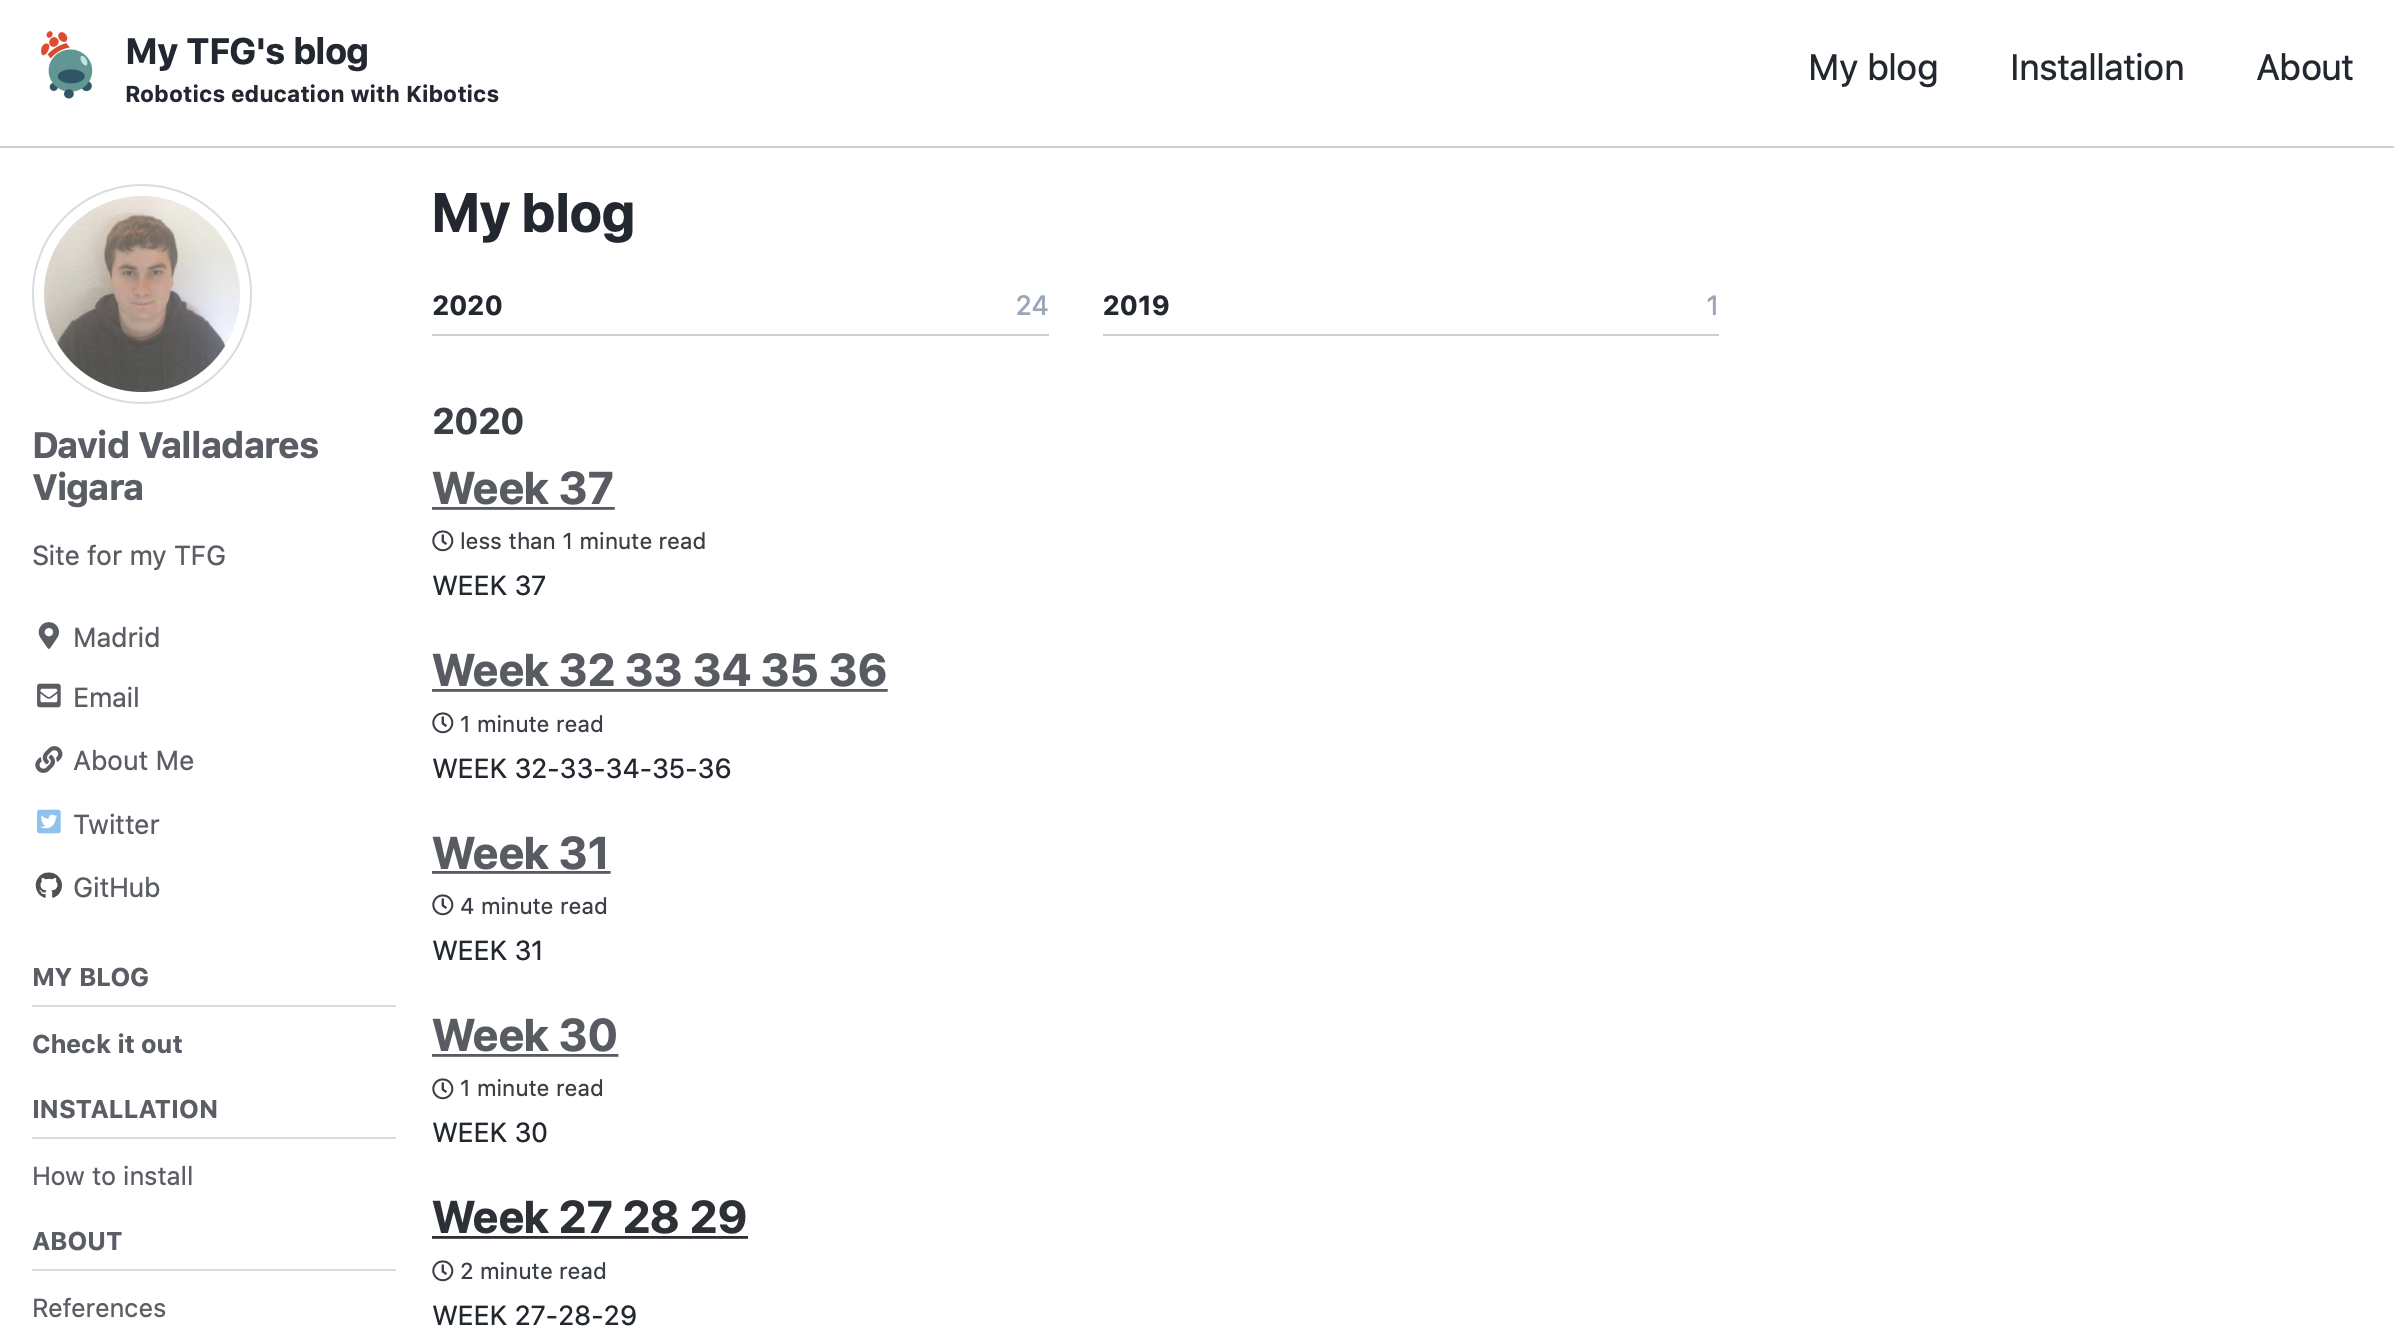
\includegraphics[width=1\textwidth]{images/blog.png}
  \caption{Blog para el seguimiento del TFG}
  \label{Blog para el seguimiento del TFG}
\end{figure}

\section{Plan de trabajo}

El plan de trabajo que se ha seguido durante la elaboración del proyecto puede dividirse en las siguientes etapas:
\begin{itemize}
	\item \textit{\textbf{Aterrizaje en la plataforma de Kibotics.}} Esta plataforma está montada usando la tecnología Django, por lo que se tuvo que aterrizar en cómo consistía el funcionamiento de esta aplicación.
	\item \textit{\textbf{Diseño para el Mbot.}} En el inicio de esta fase fue fundamental entender el Api del Web Serial y de las características del propio robot. Se hizo un primer prototipo de ejemplo para ver la interacción con una placa ArduinoUno. Posteriormente, se realizó la integración en la plataforma y se perfiló la interfaz y la usabilidad del envío del programa al robot.
	\item \textit{\textbf{Diseño para el dron Tello.}} Al igual que en la fase anterior, también se empezó estudiando las características del robot y del uso de PyInstaller. La primera integración que se diseñó fue para los ordenadores con Linux y, después, se procedió con el diseño de la integración para MacOs y Windows.
	\item \textit{\textbf{Diseño para el GopiGo3.}} En este caso, además de conocer las características del robot, también fue necesario aprender a manejar la Raspberry Pi y entender la librería Flask. Se desarrolló un primer prototipo de ejemplo para encender un led en la placa Arduino vía web. Después, se realizó la integración en Kibotics y se mejoró la interfaz y usabilidad del envío del programa.
	
\end{itemize}





%###############################################################################
%############# HERRAMIENTAS ###################################################
%###############################################################################

\chapter{Herramientas}

En este capítulo se describen las herramientas que han sido utilizas para el desarrollo de este trabajo de fin de grado.

\section{Lenguaje Python}

Python es un lenguaje de programación diseñado por Guido Van Rossum y publicado en el año 1991 (Challenger, Díaz y Becerra, 2014). Es un proyecto de código abierto gestionado por Python Software Foundation, una sociedad sin ánimo de lucro. Actualmente se encuentra en su versión 3.8 (Zaforas, 2018).
\\
\\
Presenta algunas características que implican una serie de ventajas para los usuarios y que son las responsables de su gran popularidad. En primer lugar, se trata de un lenguaje multiparadigma, es decir, permite utilizar diferentes paradigmas de programación, como son la orientación a objetos, funcional o imperativa. Además, al ser un lenguaje interpretado, no necesita ser compilado ni enlazado. Posee un tipado dinámico (aunque desde la versión 3.5 puede hacerse uso del tipado estático), y es multiplataforma, lo que significa que puede ser ejecutado en diferentes sistemas operativos (Zaforas, 2018). La sintaxis de Python es más sencilla que la de otros lenguajes de programación, algo muy importante para la educación. Además, cuenta con una de las librerías más completas, comparable a la de Java y .NET (Challenger, Díaz y Becerra, 2014). Todo esto le han convertido en uno de los lenguajes de programación más utilizados en la actualidad.

\section{Lenguaje HTML}

HTML (HyperText Markup Languaje) fue desarrollado en 1991 por Tim Berners-Lee mientras trabajaba en la Organización Europea para la Investigación Nuclear (CERN), y popularizado por el navegador Mosaic desarrollado en NCSA (Raggett, Le Hors y Jacobs, 1999).
\\
\\
No es un lenguaje de programación, es decir, no tiene capacidad de crear una funcionalidad dinámica, sino que consiste en un lenguaje de marcado de hipertexto, basado en el metalenguaje SGML (Standard Generalized Markup Language). Este lenguaje da formato a los documentos de la WWW (World Wide Web) (Lamarca, 2018). Se podría considerar un lenguaje entendido universalmente por todos los ordenadores que permite que la información publicada tenga una distribución global (Raggett, Le Hors y Jacobs, 1999).
\\
\\
La organización W3C (World Wide Web Consortium) es quien lleva a cabo las especificaciones relativas a este lenguaje. Está definido por “etiquetas” que el navegador interpreta y da forma en la pantalla. Estas etiquetas encierran un contenido y, todo en conjunto, forman lo que se denomina “elemento” (Lamarca, 2018).
\\
\begin{lstlisting}[frame=single,breaklines=true, label=Ejemplo de código HTML, caption=Ejemplo de código HTML, captionpos=b]
<!DOCTYPE html>
<html>
  <head>
    <meta charset="utf-8">
    <title>Mi pagina de prueba</title>
  </head>
  <body>
    <img src="images/firefox-icon.png" alt="Mi imagen de prueba">
  </body>
</html>

\end{lstlisting}

\section{Lenguaje JavaScript}

JavaScript es un lenguaje de programación desarrollado por Brendan Eich a finales de los años 90. Se considera un lenguaje interpretado, de tipado débil y dinámico, y se utiliza, principalmente, para crear páginas web dinámicas en el lado del cliente, es decir, aquellas que incluyen efectos, animaciones, ventanas emergentes… (Eguíluz, 2009). Sin embargo, actualmente también existe la posibilidad de ejecutar JavaScript en todo tipo de desarrollo de aplicaciones (NodeJs).
\\
\\
Su nombre se debe a que los programas o aplicaciones creados con este lenguaje de programación se denominan “script” (Eguíluz, 2009). Además, su sintaxis es muy similar a la de otros lenguajes (Java y C)

\section{Bootstrap}

Bootstrap (Figura 3.1) fue diseñado por Mark Otto y Jacob Thornton para crear mejores herramientas internas en Twitter, aunque en agosto de 2011 pasó a ser de código abierto, lo que favoreció su desarrollo (Cumplido, 2018).
\\
\\
Consiste en un framework utilizado para el desarrollo web basado en CSS (Cascading Style Sheets), un lenguaje que permite estructurar y componer páginas web, y JQuery, una librería de JavaScript utilizada para dotar de interactividad a una web. Utiliza un sistema de rejillas (cuadrículas) para el diseño de la web. Este framework facilita la tarea de maquetar una página web, creando así una interfaz muy limpia y adaptable al tamaño de la pantalla del dispositivo. Es compatible con los principales navegadores (Firefox, Google Chrome, Safari), lo que supone una gran ventaja. Además, existe una gran cantidad de documentación disponible, lo que facilita su uso y comprensión (Guevara, s.f.).
\\
\begin{figure}[h!]
  \centering
    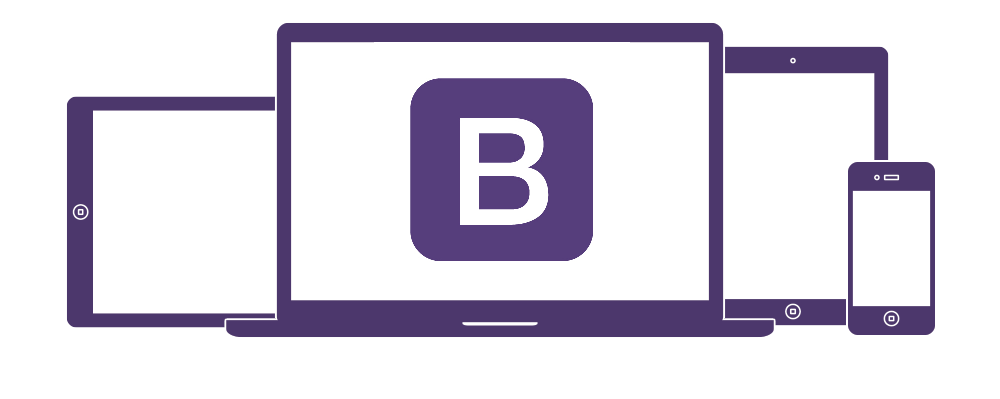
\includegraphics[width=0.5\textwidth]{images/bootstrap.png}
  \caption{Bootstrap}
  \label{Bootstrap}
\end{figure}

\section{Django}

Django es un framework de código abierto escrito en Python, creado en 2005, el cual permite desarrollar un entorno web complejo de una forma rápida y estructurada. Actualmente es mantenido por Django Software Foundation y se encuentra en la versión 3.0 (Novapros, 2020).
\\
\\
Sigue una arquitectura MVC (Modelo – Vista - Controlador), como se observa en la figura 3.2 (Holovaty y Kaplan-Moss, 2007).
\begin{itemize}
	\item \textit{Modelo}. Los modelos de datos creados están mapeados directamente a las tablas de la base de datos, permitiendo aislar el código de la aplicación de la base de datos.

	\item \textit{Vista}. Corresponde con la capa de presentación, y está basada en plantillas HTML.		
	\item \textit{Controlador (en Django llamado “views”)}. Responsable de seleccionar la plantilla a mostrar. Atiende a una petición y, según el mapeo de la URL, (Uniform Resource Locator) redirige a una vista u otra.
\end{itemize}
Ofrece una serie de características bastante interesantes como es su excelente capa de seguridad (p ej. permite una protección contra los ataques maliciosos “Cross-site request forgery”), dispone de un sistema de administrador “por defecto,” sin necesidad de realizar ningún tipo de configuración. También proporciona una interfaz para el acceso a la base de datos, facilitando las consultas (Novapros, 2020).
\begin{figure}[h!]
  \centering
    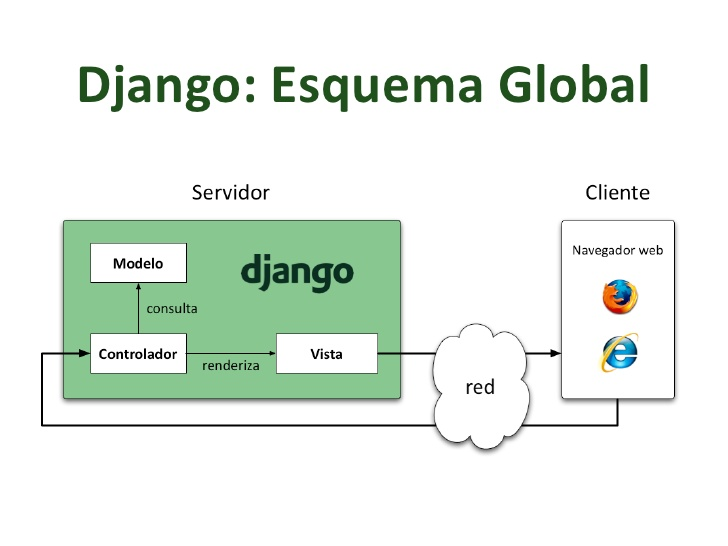
\includegraphics[width=0.6\textwidth]{images/django.png}
  \caption{Arquitectura Django}
  \label{Arquitectura Django}
\end{figure}

\section{Flask}

Flask (Figura 3.3), lanzado en abril de 2010 es, junto con Django, uno de los framework webs más famosos escritos en Python.
\\
\\
Está enfocado en proporcionar lo mínimo necesario para poner en funcionamiento una aplicación, por eso se le considera un framework “minimalista”. Por otro lado, no requiere de otras dependencias para realizar acciones básicas, de manera que la curva de aprendizaje para su comprensión es muy baja. Debido a su sencillez en la estructura, posee una velocidad mayor que Django y es bastante útil para iniciarse en el aprendizaje de desarrollo web, permitiendo crear servidores de una forma rápida. Debido a ello, Flask está orientado al sector servicios, los cuales implican muchas visitas y una carga grande de peticiones, y también para proyectos personalizados o sencillos (Rodríguez, 2019).
\begin{figure}[h!]
  \centering
    
\includegraphics[width=0.4\textwidth]{images/flask.png}
  \caption{Arquitectura Django}
  \label{Arquitectura Django}
\end{figure}

\section{Web Serial Api}

Web Serial es una Api (Application Programming Interface) JavaScript, especificada por WICG (Web Platform Incubator Community Group), que permite interactuar con dispositivos conectados al puerto serie del ordenador desde un navegador web. Actualmente esta Api es soportada por los navegadores de escritorio basados en Chromium (Google Chrome, Opera, Edge), pero para poder utilizarla es necesario habilitarla.
\\
\\
Muchos dispositivos periféricos que se conectan al ordenador requieren de una descarga software para controlarlo. Un claro ejemplo de esto se ve en la robótica; en la mayoría de los robots en los que la carga del programa se realiza por USB (Universal Serial Bus), es necesario instalar previamente en el ordenador un software que permita hacerlo. La ventaja de Web Serial es que  proporciona una vía capaz de comunicarse con estos dispositivos sin necesidad de instalar nada en el ordenador (W3C Community Group, 2020).

\section{PyInstaller}

PyInstaller es un módulo lanzado por la línea de comandos que permite agrupar aplicaciones Python en un único paquete junto con todas las dependencias necesarias y el intérprete de Python, permitiendo crear un ejecutable para ser distribuido. Es compatible con las versiones de Python 2.7 y para las versiones superiores a Python3.3. Puede ser utilizado para Linux, Windows y MacOs, aunque no permite una compilación cruzada, es decir, la aplicación empaquetada solo puede utilizarse en el mismo sistema operativo en el que fue empaquetado, por lo que una aplicación empaquetada en Linux no podrá ser utiliza en una computadora con Windows o MacOs (SO Documentation, s.f.).
\\
\begin{lstlisting}[frame=single,breaklines=true, label=Ejemplo para generar un ejecutable con PyInstaller, caption=Ejemplo para generar un ejecutable con PyInstaller, captionpos=b]
 		   $ pyinstaller -onefile hello.py
\end{lstlisting}

\section{Placa mCore}

La placa mCore (Figura 3.4) está basada en una placa ArduinoUno, una microcontroladora de código abierto que utiliza un microchip ATmega328P, pero extendida con más componentes y que, además, incorpora la electrónica de potencia para el manejo de los motores.
\\
\begin{figure}[h!]
  \centering
    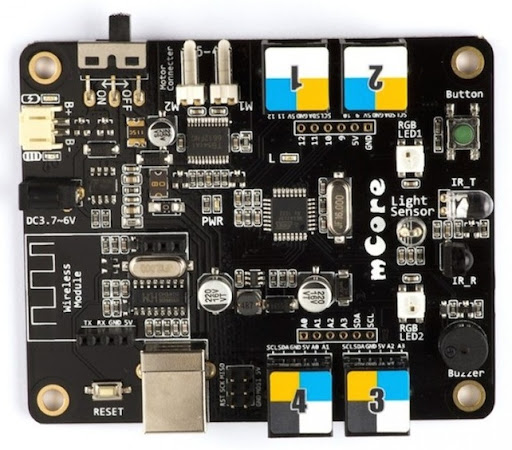
\includegraphics[width=0.5\textwidth]{images/mcore.png}
  \caption{Placa mCore}
  \label{Placa mCore}
\end{figure}
\\
La placa permite ser programada a través del puerto serie gracias al bootloader, un software alojado en la memoria flash. En el arranque de la placa, el bootloader comprueba si se está intentado programarla y, en caso afirmativo, se procede a grabar el programa en la memoria y se reinicia. En el caso contrario, el bootloader ejecuta el último programa que estuviera grabado. Estas placas pueden ser programadas utilizando el lenguaje Arduino, un lenguaje de alto nivel que está basado en el lenguaje C++, pero adaptado para facilitar la programación de los pines de entrada y salida (Llamas, 2016).
\\
\\
Una vez que el programa ha sido escrito en este lenguaje de alto nivel, es necesario compilarlo para obtener el código ejecutable entendido por la placa para el proceso de carga (Figura 3.5).
\\
\begin{figure}[h!]
  \centering
    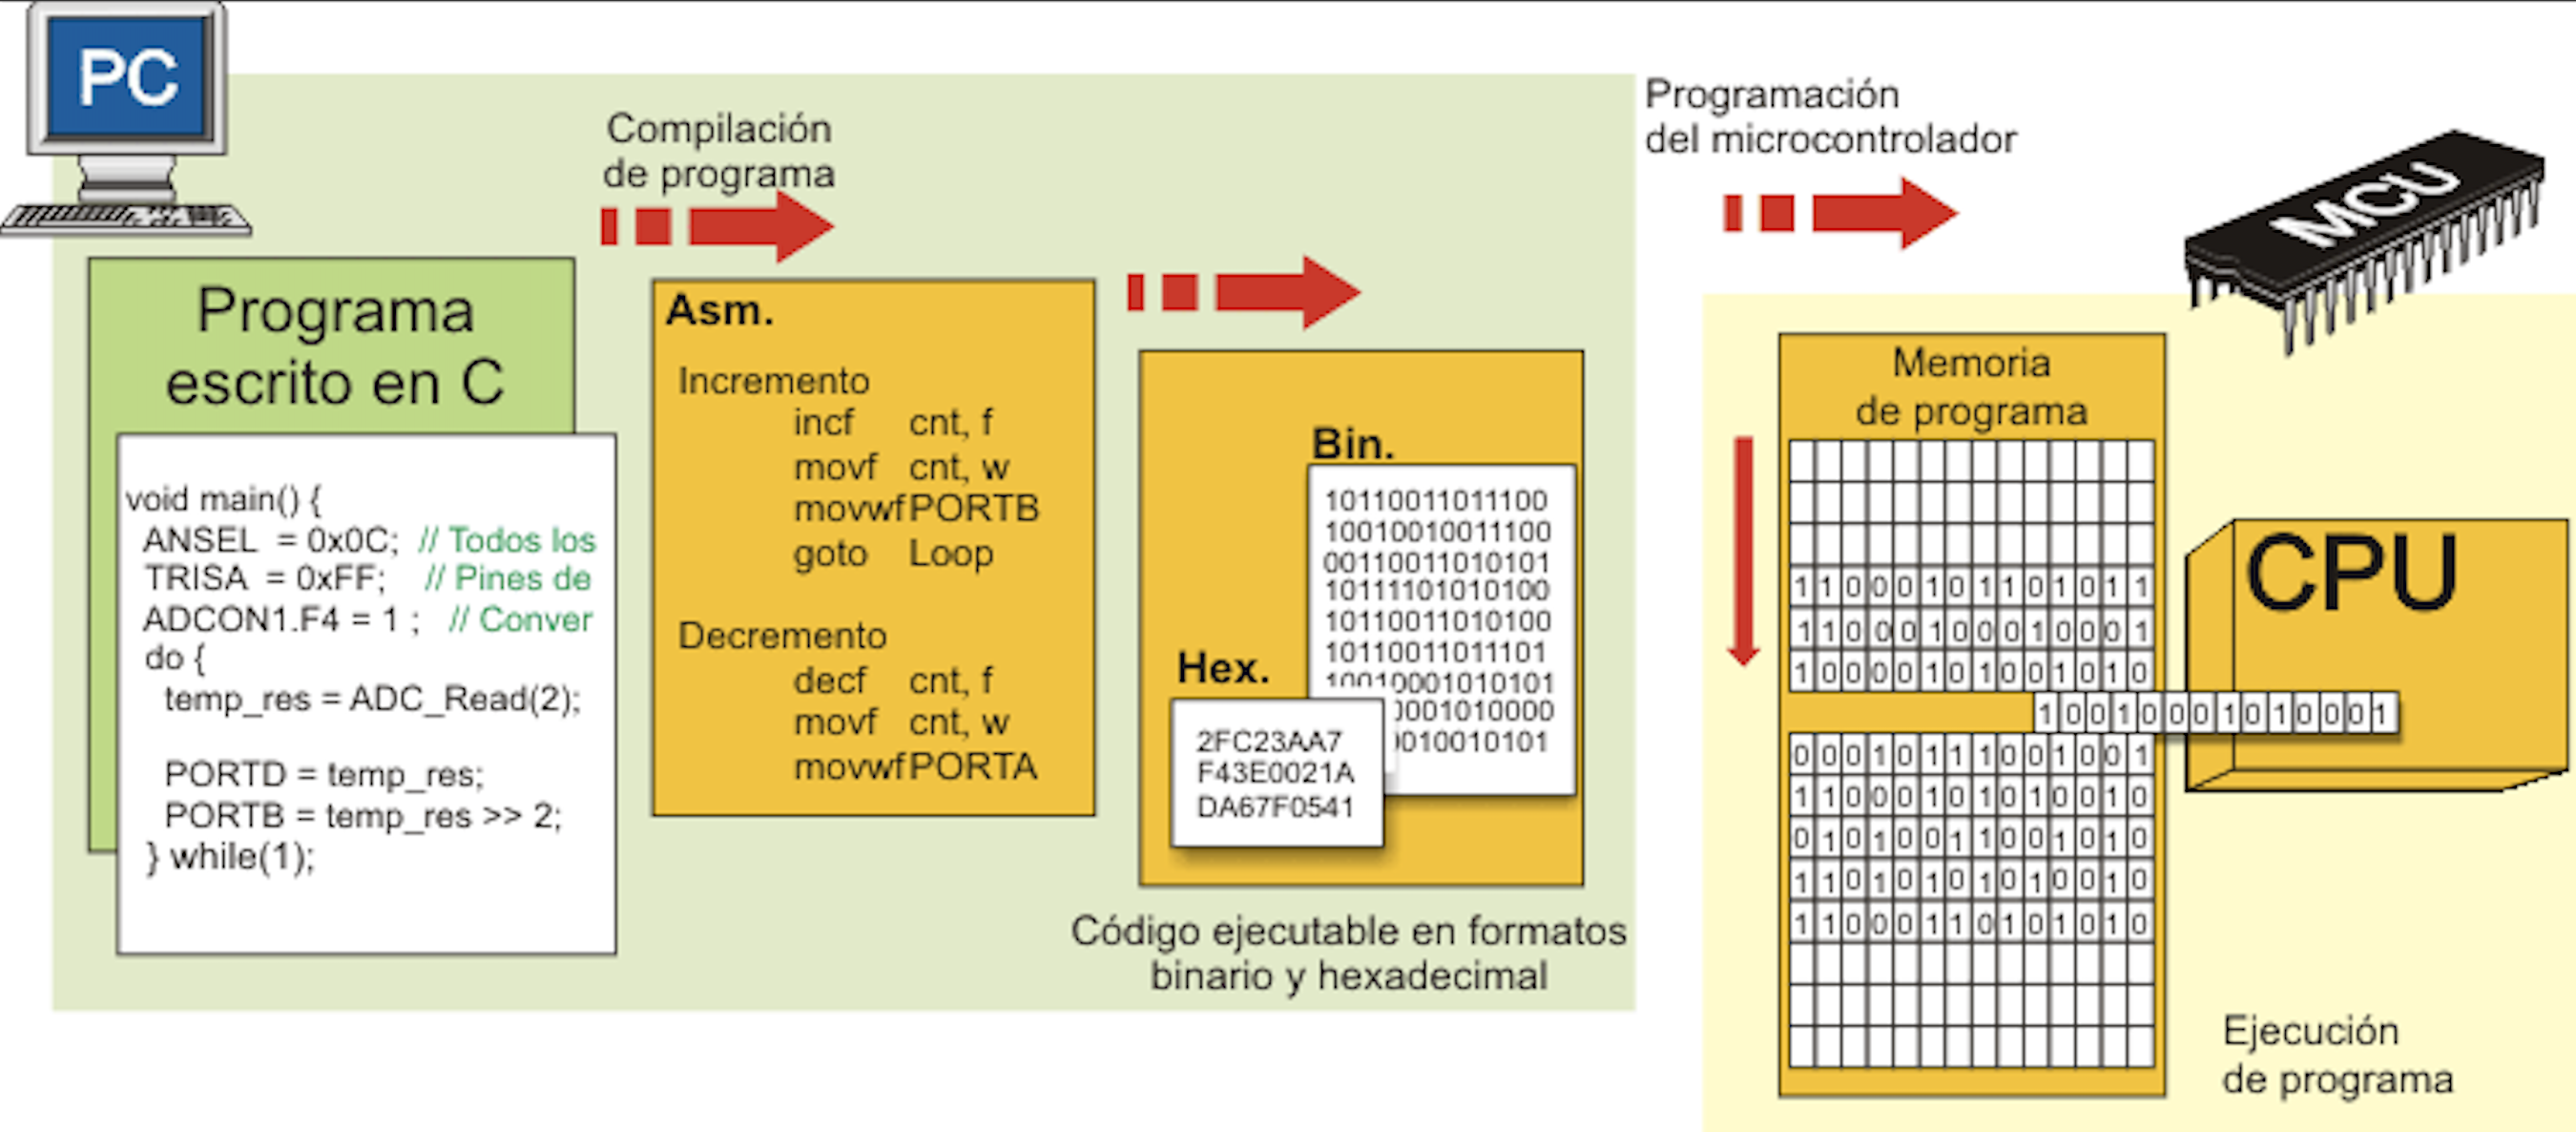
\includegraphics[width=1\textwidth]{images/carga_mcore.png}
  \caption{Proceso de carga de un programa a la placa mCore}
  \label{Proceso de carga de un programa a la placa mCore}
\end{figure}

\section{Raspberry Pi}

Raspberry Pi es un proyecto que nace en 2009 en Londres bajo la asociación caritativa denominada Fundación Raspberry Pi, cuyo objetivo era mejorar la enseñanza de la informática en las aulas.
\\
\\
Consiste una placa computadora de bajo coste que puede considerarse como un ordenador de tamaño reducido. Su hardware se compone, principalmente, de una CPU (Central Processing Unit), una GPU (Graphics Processing Unit), una memoria RAM (Random Access Memory), una ranura SD (Secure Digital) utilizada para el almacenamiento, salidas y entradas de audio y vídeo, pines de entrada y salida de propósito general (GPIO), bus USB, tarjeta de red y alimentación. En cuanto a su software, existen una gran cantidad de sistemas operativos que pueden usarse, tales como  Raspbian, Kali Linux, Windows 10 IoT Core, Ubuntu Core… (Escuela Técnica Superior de Ingeniería Informática de la Universidad Politécnica de Valencia, 2013).
\\
\\
Este ordenador es muy utilizado en la actualidad gracias a la gran variedad de usos que puede ofrecer, ya que puede emplearse como un ordenador de sobremesa, utilizarse en Robótica, como un dispositivo para la domótica…
\\
\\
Para este TFG, hemos usado la Raspberry Pi 3 modelo B. En la figura 3.6 se muestran sus características principales.
\\
\begin{figure}[h!]
  \centering
    \includegraphics[width=1\textwidth]{images/hardware_RaspberryPi.png}
  \caption{Características hardware para la Raspberry Pi modelo 3B}
  \label{Características hardware para la Raspberry Pi modelo 3B}
\end{figure}














%###############################################################################
%###################### MBOT ###################################################
%###############################################################################

\chapter{Integracion Mbot en Kibotics}
En este capítulo se aborda el proceso de integración que va a permitir programar al robot físico Mbot sin necesidad de una instalación previa ni descargas adicionales.

\section{Características del Mbot}

Mbot es un robot fácil de montar y con una estructura robusta, orientado para empezar el aprendizaje de la robótica y la programación desde la educación primaria. Está diseñado por la empresa MakeBlock, la cual dispone de una gran variedad de recursos, robots y kits de robotica.
\\
\\
El robot pesa 400 gramos y sus dimensiones son de 17x13x9 cm. Respecto a las especificaciones técnicas, posee una placa llamada “mCore” que está basada en ArduinoUno, dispone de una microcontroladora ATmega238, cuatro puertos Rj25, un interruptor de encendido, dos leds RGB, un botón, zumbador, un sensor de infrarrojos y otro de luminosidad. Dispone de una batería de litio de 3,7V, pero también funciona con cuatro pilas de tipo AA. En cuanto  sus módulos externos, presenta dos motes, ultrasonido y un seguidor en línea, aunque también pueden utilizarse otras conexiones adicionales. Se comunica por vía puerto serie o por Bluetooth 4.0 (Robótica Educativa con Mbot, 2020).
\\
\begin{figure}[h!]
  \centering
    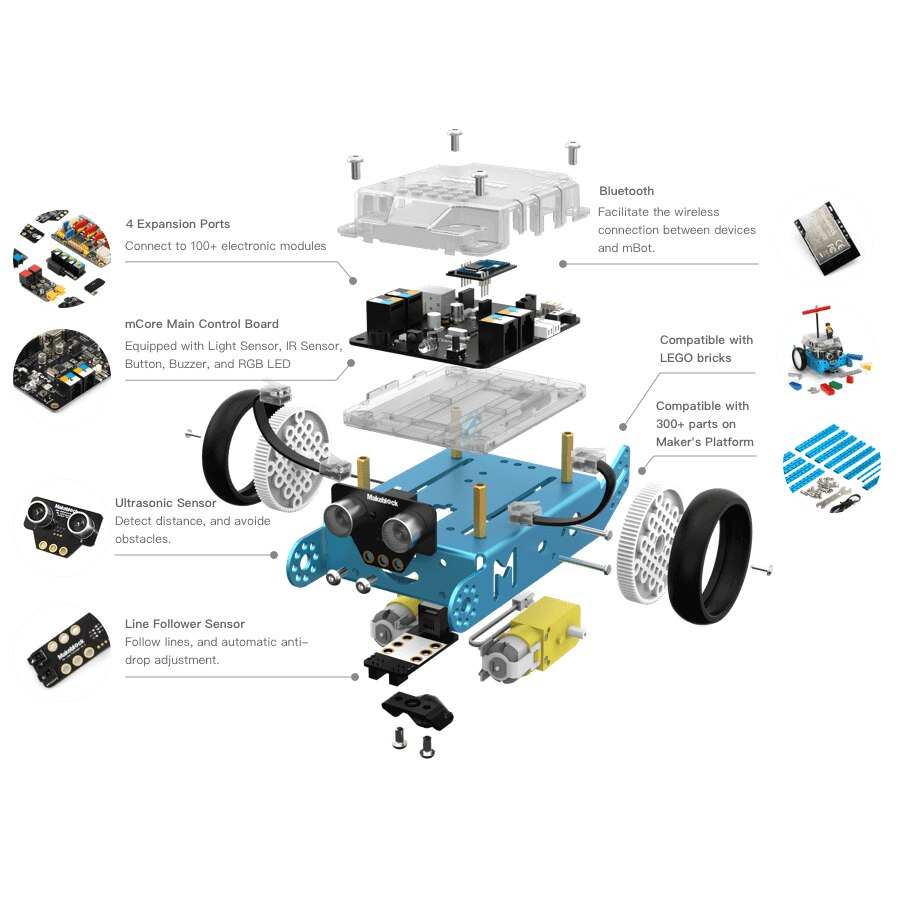
\includegraphics[width=1\textwidth]{images/partes_mbot.png}
  \caption{Partes robot Mbot}
  \label{figura:Partes robot Mbot}
\end{figure}
\\
MackeBlock distribuye un software gratuito, llamador mBlock (Figura 4.2) que permite programar a este robot. Este software puede ser usado vía web, aunque para utilizarlo de esta manera es necesario que el usuario instale un driver, también puede utilizarse de forma local, descargándolo en el ordenador. Con él se puede programar al Mbot utilizando los lenguajes de programación Scratch o Python.
\\
\begin{figure}[h!]
  \centering
    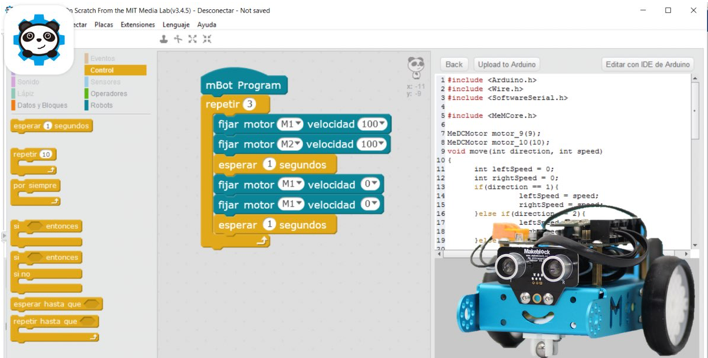
\includegraphics[width=1\textwidth]{images/software_mBlock.png}
  \caption{Software mBlock}
  \label{Software mBlock}
\end{figure}

\section{Diseño}

En la Figura 4.3 se muestra el diseño seguido para la integración del Mbot en la plataforma de Kibotics.
\\
\begin{figure}[h!]
  \centering
    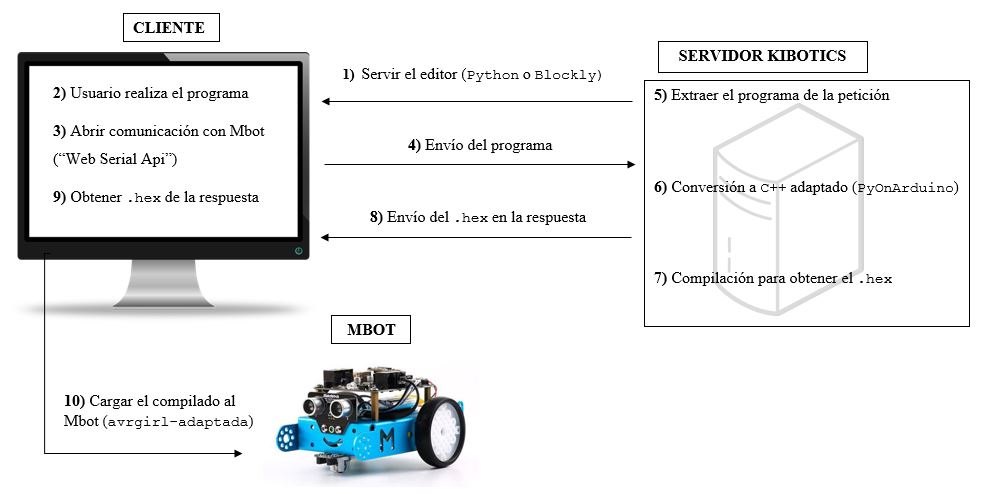
\includegraphics[width=1\textwidth]{images/infraestructura_mbot.png}
  \caption{Infraestructura seguida para la integración del Mbot}
  \label{Infraestructura seguida para la integración del Mbot}
\end{figure}
\\
En las secciones siguiente se detallarán cuales son las interacciones necesarias entre el cliente y el servidor para permitir la carga del programa al Mbot

\section{Lado Cliente}

Desde la parrilla principal de Kibotics se puede entrar a la unidad dedicada al Mbot, pudiendo elegir qué lenguaje de programación usar (Python o Blockly). Dentro de dicha unidad encontramos un apartado dedicado a proporcionar las instrucciones necesarias para realizar un programa y enviárselo al Mbot. 
\\
\\
Gracias al diseño utilizado, no es necesario que el usuario instalé nada en su ordenador ni en el robot para permitir su uso, por lo que el proceso de programación del robot se limitará a que una vez que el usuario ha realizado el programa se envié al robot directamente.

\subsection{Editor}

En la unidad del robot se proporciona un editor que le permitirá al usuario escribir el programa que será enviado al robot. Según la unidad elegida el editor estará orientado a ese lenguaje.
\\
\begin{figure}[h!]
  \centering
    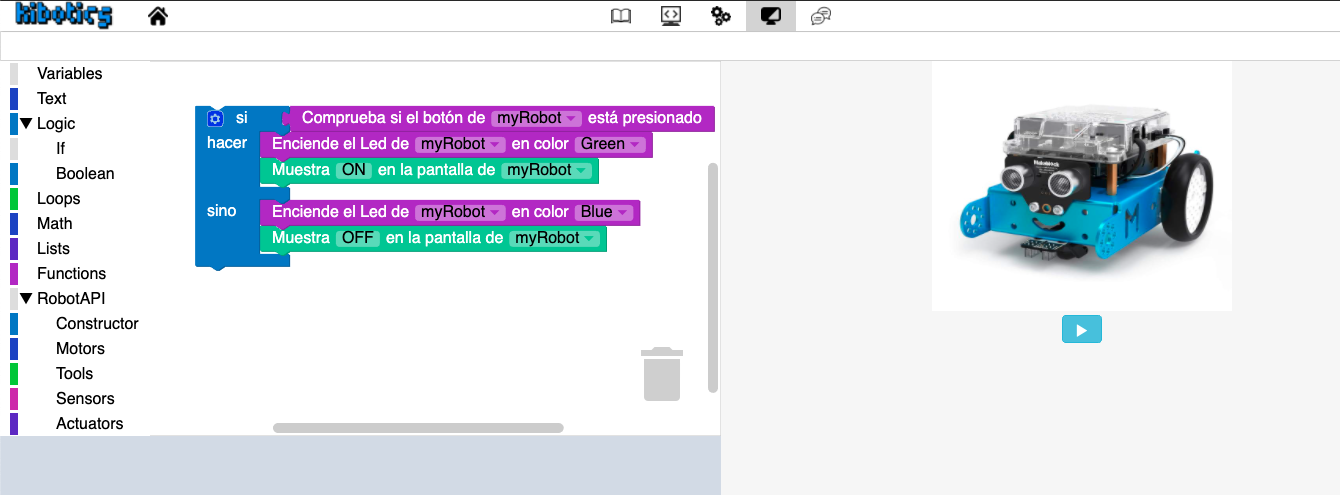
\includegraphics[width=0.9\textwidth]{images/editor_mbot.png}
  \caption{Editor Blockly para el Mbot }
  \label{Editor Blockly para el Mbot }
\end{figure}
\\

\subsection{Conexión con el Mbot (USB)}

Una vez que el usuario ha realizado el programa deseado y ha conectado el Mbot por USB a su ordenador, al pulsar el botón azul que se muestra en la Figura 4.4, se iniciará el proceso de envío.
\\
\\
En primer lugar, se abrirá una ventana que muestra los puertos del ordenador disponibles. Se debe seleccionar en el que se encuentra conectado el robot, que aparece nombrado como USB2.0Serial. Esta acción permitirá abrir una comunicación entre el navegador y el robot (Fragmento 4.1). Esto es posible gracias a “Web Serial Api”, que proporciona una Api al navegador capaz de interactuar con el puerto serial de la computadora.
\\
\begin{lstlisting}[frame=single,breaklines=true, label=Abrir conexión con el Mbot por el puerto serie, caption=Abrir conexión con el Mbot por el puerto serie, captionpos=b]  % Inicia el bloque de código
   document.addEventListener('DOMContentLoaded', () => {

      document.getElementById('uploadMbot').addEventListener('click', clickConnect);

   });

   async function clickConnect() {
      progress.style.width = '0%';
      alertError.style.visibility = 'hidden';
      //-- Si el puerto serie estaba ya abierto, cerrarlo
      if (portPrev) {
         await disconnect();
      }
      await connect();
      activeProgress.style.visibility = 'visible';
      progress.style.width = '25%';
      if(document.getElementById('uploadMbot').value == 'python'){
          send_code_to_mbot()
      }else{
          convert_and_send_code_to_mbot();
      }

   }

   async function connect() {
      portPrev = await navigator.serial.requestPort();

      await portPrev.open({ baudrate: 115200 });

   }
   async function disconnect() {
       // -- Cerrar el puerto serie
      await portPrev.close();
      portPrev = null;
   }
\end{lstlisting}


\subsection{Envío del código fuente al servidor}

Una vez abierta la comunicación de forma correcta, se procede a enviar el programa desde el navegador a el servidor de Kibotics, para su manipulación, como un query parameter de una petición GET. Para este envío se utiliza la función fetch() que está proporcionada por JavaScript (Fragmento 4.2).
\\
\begin{lstlisting}[frame=single,breaklines=true, label=Envio del programa desde el navegador al servidor, caption=Envio del programa desde el navegador al servidor, captionpos=b]
   function send_code_to_mbot() {
      var editor = ace.edit("ace");
      let code = editor.getValue();
      console.log(code);
      var enc = new TextEncoder();
      const message = {
         method: "GET"
       };
       url = '/get_python_to_arduino_binary?python_code=' + JSON.stringify(code);
       fetch(url, message)
             . . . . .
  
 }
\end{lstlisting}
Hay que tener en cuenta que si el programa está escrito en Blockly, debe convertirse previamente al lenguaje Python antes de enviarse, como puede verse en el fragmento 4.3.
\\
\begin{lstlisting}[frame=single,breaklines=true, label=Conversión de Blockly a Python, caption=Conversión de Blockly a Python, captionpos=b]
   var pythoncode = Blockly.Python.workspaceToCode(editor.ui);
\end{lstlisting}

\subsection{Recepción del ejecutable}

De la respuesta enviada por el navegador con el programa realizado al servidor, se recibe una respuesta que contiene el programa compilado para poder enviárselo a la microcontroladora.
\\
\\
La función fetch(), mencionada anteriormente, espera hasta recibir la respuesta, pudiendo extraer así el cuerpo de la respuesta, donde se encuentra la compilación del programa.
\\
\begin{lstlisting}[frame=single,breaklines=true, label=Extracción del dato enviado en la respuesta, caption=Extracción del dato enviado en la respuesta, captionpos=b]
   fetch(url, message)
      .then(function(response) {
         if(response.ok){
            responseOk = true
         }else{
            responseOk = false
         }
           return response.text();
      })
      .then(function(data) {
        
         var dataBuffer = enc.encode(data);
           
      })
      .catch(function(err) {

         console.error(err);
       });

\end{lstlisting}


\subsection{Carga en el robot y ejecución}

Una vez extraído el código compilado, se procede a cargarlo en el robot. Avrgirl-arduino, una librería nodejs de código abierto, proporciona esa posibilidad de quemar el programa compilado a la microcontroladora, y es compatible con un gran número de placas (entre ellas ArduinoUno). Hemos utilizado esta librería adaptándola a nuestras necesidades para el proceso de carga.
\\
\begin{lstlisting}[frame=single,breaklines=true, label=Carga del compilado al Mbot, caption=Carga del compilado al Mbot, captionpos=b]
   . . . 
   
   .then(function(data) {

      if(responseOk){
         var dataBuffer = enc.encode(data);
         upload_to_mbot(dataBuffer)
         progress.style.width = '99%';
         alertError.style.visibility = 'hidden';
      }else{
         console.log("Fallo al compilar el programa")
         infoError.innerHTML = "Error"
         alertError.style.visibility = 'visible';
         activeProgress.style.visibility = 'hidden';
      }

   })
    . . . 
    
    function upload_to_mbot(dataBuffer){
       let avrgirl = new AvrgirlArduino({
          board: "uno"
       });

       avrgirl.flash(dataBuffer,(error) =>  {
          if (error) {
             console.error(error);
             portPrev = null;
             infoError.innerHTML = "Error!"
             alertError.style.visibility = 'visible';
             activeProgress.style.visibility = 'hidden';

          } else {
             console.info('done correctly.');
             portPrev = null
             alertError.style.visibility = 'hidden';
             activeProgress.style.visibility = 'hidden';
          }
      });
   }

\end{lstlisting}
Tras “quemar” el programa en el Mbot, este empezará a ejecutar las instrucciones que le fueron programadas.

\section{Lado Cliente}

El servidor de Kibotics es el encargado de servir al navegador las páginas que le permiten ir navegando por la web, y por lo tanto dirigirse a la unidad del Mbot. Pero también toma otro papel fundamental para el desarrollo del envió, ya que será el responsable de adaptar el código que el usuario ha escrito, para que pueda ser entendido por la controladora del robot a la hora de realizarse la carga.

\subsection{Recepción del código fuente}
Una vez que el usuario realizo su programa y pulso en enviar, el navegador le envía al servidor el código escrito para que este lo adapte. Por lo que el servidor tendrá que extraer el código (Fragmento 4.6), que se encuentra en un \textit{query parameter} de la URL.
\\
\begin{lstlisting}[frame=single,breaklines=true, label=Extracción del programa en el servidor, caption=Extracción programa en el servidor, captionpos=b]
   def get_python_to_arduino_code_binary(request):
      . . . .
      python_code = json.loads(request.GET.get('python_code', None))
      . . . .

\end{lstlisting}

\subsection{Conversión}

El programa extraído en el servidor es lenguaje Python, pero el Mbot, basado en Arduino, no entiende este lenguaje. El lenguaje de alto nivel que usa Arduino, para posteriormente generar el compilado que entiende, es un C++ adaptado, por lo que se debe traducir desde Python. Esto es posible gracias a la librería PyOnArduino, la cual proporciona los mecanismos necesarios para esa traducción y conversión de un fichero.py (extensión para Python) a .ino (extensión para Arduino).
\\
\begin{lstlisting}[frame=single,breaklines=true, label=Traducción de lenguaje Python a Arduino, caption=Traducción de lenguaje Python a Arduino, captionpos=b]
   . . .    
    parsed_file = ast.parse(code)
    translator.robot = 'MBot'
    translator.robot_architecture = ''
    translator.vars.Variables()
    translator.vars.halduino_directory = py_to_arduino_path + 'HALduino/halduino'
    translator.TranslatorVisitor().visit(parsed_file)
    translator.create_setup()
    translator.variables_manager = translator.create_variables_manager(file=py_to_arduino_path + 'HALduino/variablesManager.ino')
    translator.create_output('output-file.ino')
    translator.create_makefile('MBot', py_to_arduino_path + 'makefiles/')
    . . .


\end{lstlisting}


\subsection{Compilación cruzada}

Una vez extraído el código, se debe compilar para obtener el fichero .hex que contiene las instrucciones traducidas a hexadecimal entendidas por la microcontroladora. Esta compilación se lleva a cabo utilizando avrdude, una herramienta que permite la programación de chips AVR y que puede ser llamada por la línea de comandos.
\\
\begin{lstlisting}[frame=single,breaklines=true, label=Compilado y obtención del .hex, caption=Compilado y obtención del .hex, captionpos=b]
def create_mbot_binary():
    shutil.copyfile(os.path.join(settings.BASE_DIR, 'kibotics-drivers/mbot/avrdude'), './avrdude')
    shutil.copyfile(os.path.join(settings.BASE_DIR, 'kibotics-drivers/mbot/libftdi1.so'), './libftdi.so')
    shutil.copyfile(os.path.join(settings.BASE_DIR, 'kibotics-drivers/mbot/libreadline.so'), './libreadline.so.6')
    shutil.copyfile(os.path.join(settings.BASE_DIR, 'kibotics-drivers/mbot/avrdude.conf'), './avrdude.conf')
    shutil.copytree(os.path.join(settings.BASE_DIR, 'kibotics-drivers/mbot/arduino-1.8.10/'), 'arduino/')
    call(['make'])
    exercise_dir = './'
    # Extraemos el binario
    f_binary = open(exercise_dir + 'build-uno/output.hex', 'r')
    binary = f_binary.read()
    f_binary.close()
    return binary
\end{lstlisting}

\subsection{Envío del ejecutable}

Tras la compilación del programa, obtenemos el.hex, que será enviado como respuesta al navegador, para que pueda ser cargado al robot.
\\
\begin{lstlisting}[frame=single,breaklines=true, label=Respuesta a la petición que envió el navegador, caption=Respuesta a la petición que envió el navegador, captionpos=b]
    . . .
    binary = create_mbot_binary()

    response = HttpResponse(binary, content_type='text/plain')
    response['Content-Length'] = len(response.content)
    return response
\end{lstlisting}

\section{Validación experimental}

En las secciones anteriores no se ha mencionado en ningún momento para qué sistema operativo era compatible todo el proceso de envío, y es aquí donde recae una de las principales ventajas de este desarrollo, pues al tratarse de una tecnología de lado del navegador, proporciona compatibilidad para cualquier sistema operativo que disponga de un navegador basado en Chromium (Google Chrome, Opera, Edge), ya que actualmente Web Serial solo esta disponible para ellos. Con este diseño se permite consiguir que esta herramienta sea multiplataforma.
\\
\\
Además, al no necesitar una instalación previa de dependencias o programas por parte del usuario, su usabilidad es más sencilla. Esto es muy importante de cara al uso de la plataforma, ya que al estar orientada a alumnos de baja edad, es necesario que el proceso sea lo más simple posible.
\\
\\
La principal desventaja es que, actualmente, Web Serial Api está en fase de experimentación, por lo que necesita ser activada con un proceso previo. Para ello, para activarla por ejemplo en Chrome, debemos escribir en el navegador Chrome \textit{“chrome://flags”} y habilitar el flag \textit{“Experimental web Plataform features”}.
\\ 
\\
La integración del Mbot ha sido probada en diferentes sistemas operativos, verificando el correcto funcionamiento (\textit{Ubuntu 18.04}, \textit{Ubuntu 16.04}, \textit{Windows 10},  \textit{Windows 8},  \textit{MacOs Mojave Versión 10.14.6}).
\\
\\
Por ultimo, se han creado una serie de vídeos, donde se puede visualizar un ejemplo de realización de un programa y envío al Mbot desde la plataforma Kibotics ,para los principales sistemas operativos:
\begin{itemize}
	\item \textbf{En Linux:} \textit{https://youtu.be/1jyvoN5ZRxQ}
	\item \textbf{En Windows:}. \textit{https://youtu.be/4Wq4kMRUeIc}
	\item \textbf{En MacOs:} \textit{https://www.youtube.com/watch?v=UyNa9R-L0Ps}
\end{itemize}

\begin{figure}[h!]
  \centering
    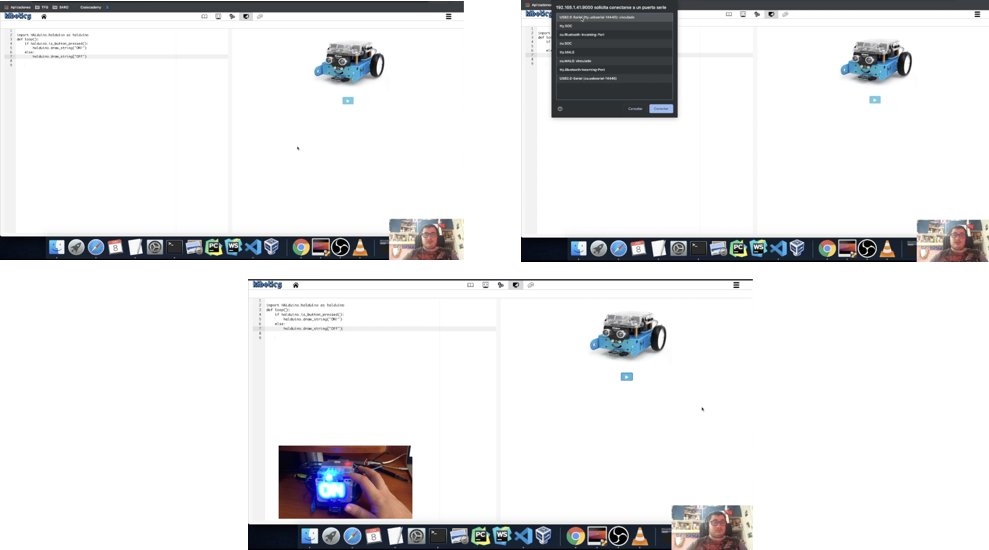
\includegraphics[width=1\textwidth]{images/fotogramas_mbot.png}
  \caption{Fotogramas del vídeo de ejemplo de envío para el Mbot en MacOs}
  \label{Fotogramas del vídeo de ejemplo de envío para el Mbot en MacOs}
\end{figure}






%###############################################################################
%###################### Tello ####################################################
%###############################################################################


\chapter{Integracion Dron Tello en Kibotics}

En este capítulo se describe el desarrollo realizado para poder programar el dron Tello. A diferencia del Mbot, donde el proceso era similar para cualquier sistema operativo, en este caso el proceso va a variar.

\section{Drone Tello}

Tello es un mini dron distribuido por la empresa Ryze Technology (Figura 5.1). Debido a la facilidad de su uso, está destinado tanto a niños como a adultos que quieran aprender a utilizar drones. Puede alcanzar una velocidad de hasta 28 km/h, su radio de control abarca hasta los 100 metros y su señal de vídeo se transmite a una frecuencia de 2,4Ghz. Posee una unidad procesadora de Intel, un barómetro para controlar de altura, motores de tipo escobilla y una cámara de 720p. Además, sus hélices están protegidas y es resistente a las caídas.
\\
\\
Entre sus puntos fuertes destacan su gran estabilidad durante el vuelo y que utiliza un sistema de posicionamiento por visión (VPS). El sistema VPS utiliza un mínimo de dos cámaras para medir la distancia al suelo y la posición a la que se encuentra, compensando así los cambios en la posición que puedan darse (Castro, 2019).
\\
\begin{figure}[h!]
  \centering
    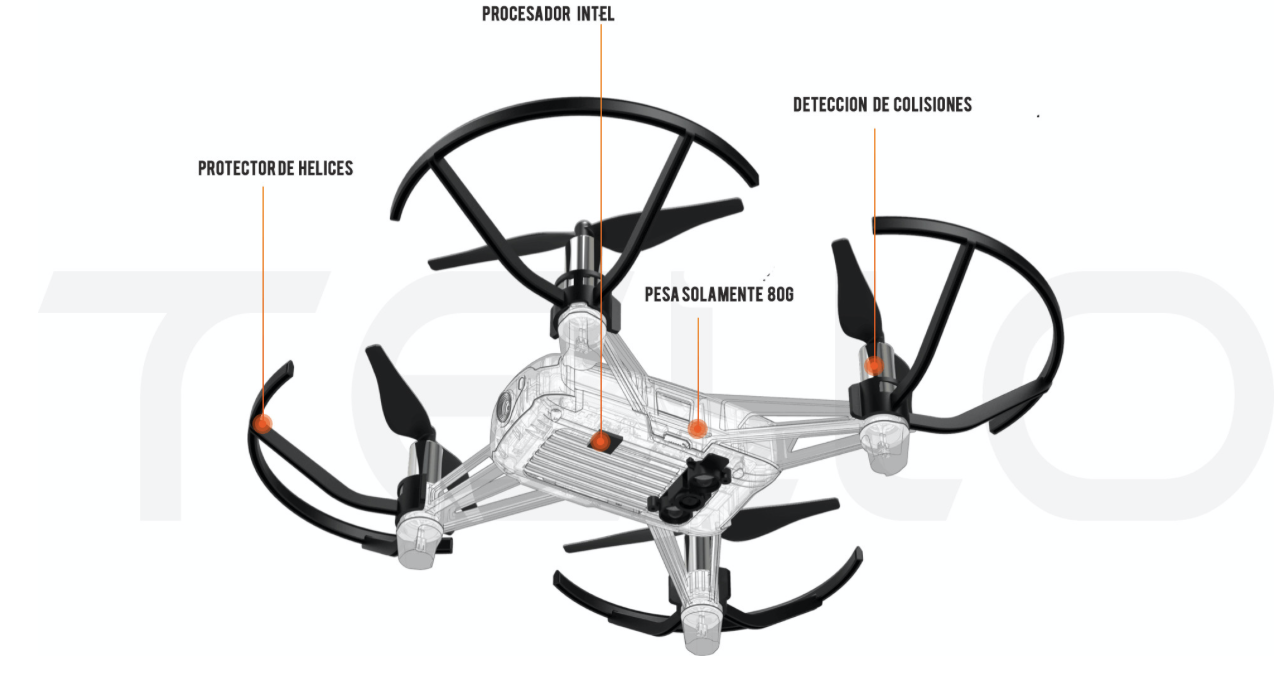
\includegraphics[width=0.9\textwidth]{images/partes_dron_tello.png}
  \caption{Esquema del dron Tello}
  \label{Esquema del dron Tello}
\end{figure}
\\
Existen una variedad de software que permiten programar al Tello, entre los que destacan.
\begin{itemize}
	\item Tello EDU App, es una aplicación diseñada para móviles o tables (Ios y Android), creada por la propia empresa que distribuye a este dron (RYZE Technology), que permite programarle utilizando bloques. Además incluye una opción para programar a un dron Tello simulado.
	\item El IDE (Integrated Development Environment) de Scratch ofrece la posibilidad de programar a este dron utilizando este lenguaje, aunque requiere para su uso, instalaciones previas en el ordenador del usuario.
	\item DroneBlocks además de permitir programar el Tello, ofrece la posibilidad de utilizar otros drones (Phantom 3, Phantom 4, Mavic Pro, Mavic Air, Spark). Utiliza también un lenguaje de bloques basado en Scracth y esta disponible en iOS App Store ,  Google Play Store y Chrome App Store.
\end{itemize}
\begin{figure}[h!]
  \centering
    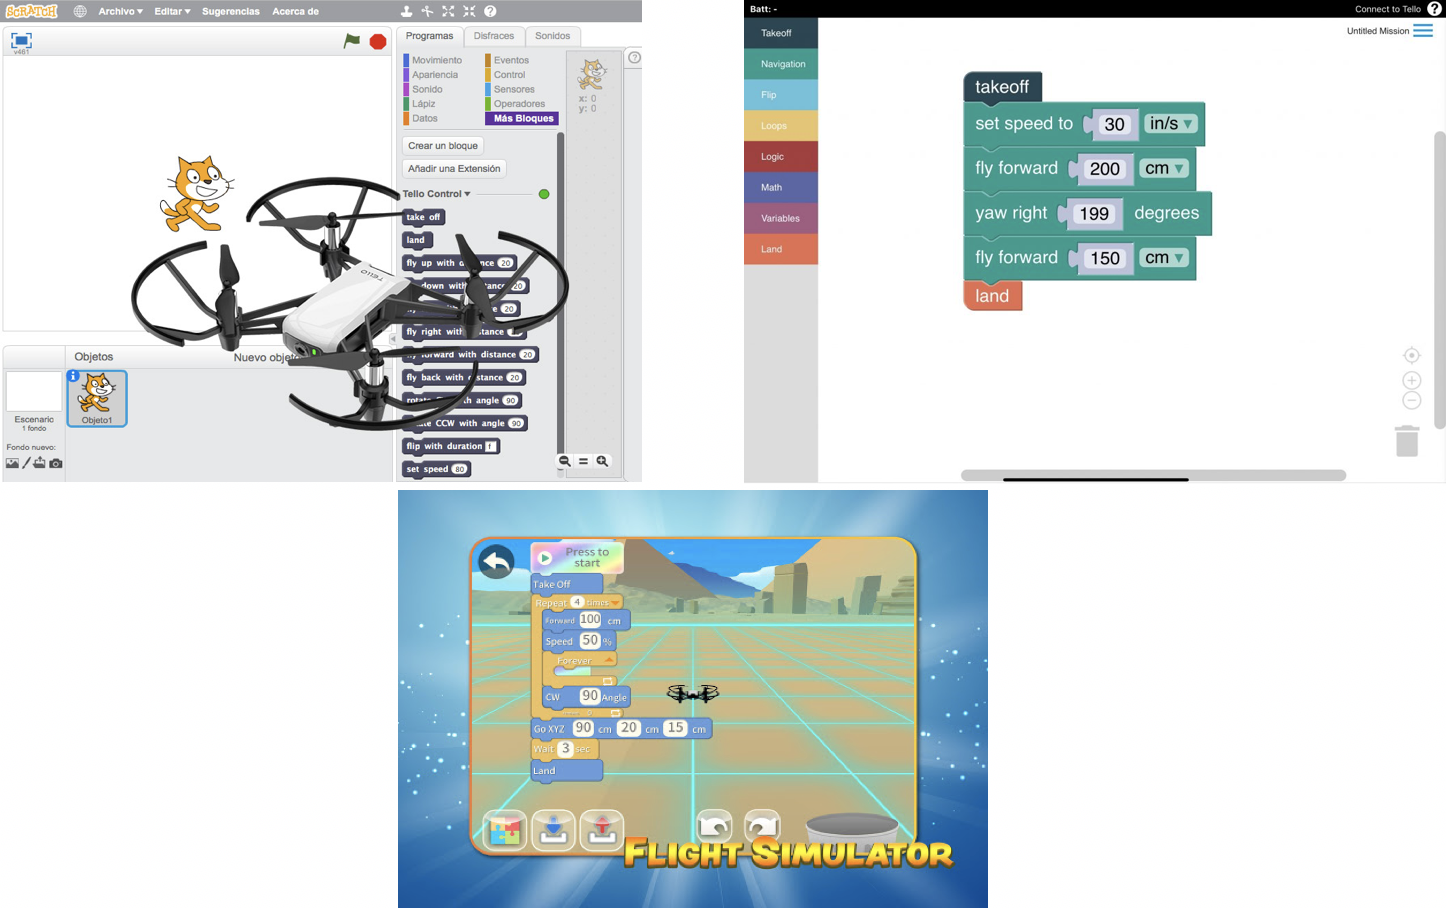
\includegraphics[width=0.9\textwidth]{images/software_tello_ide.png}
  \caption{IDE de Arduino (arriba a la izquiera), DroneBlocks (arriba a la derecha) y Tello EDU App (abajo)}
  \label{IDE de Arduino, DroneBlocks y Tello EDU App}
\end{figure}

\section{Diseño}

En la Figura 5.3, se muestra cuál es la arquitectura necesaria para conseguir el envío del programa al dron Tello.
\\
\begin{figure}[h!]
  \centering
    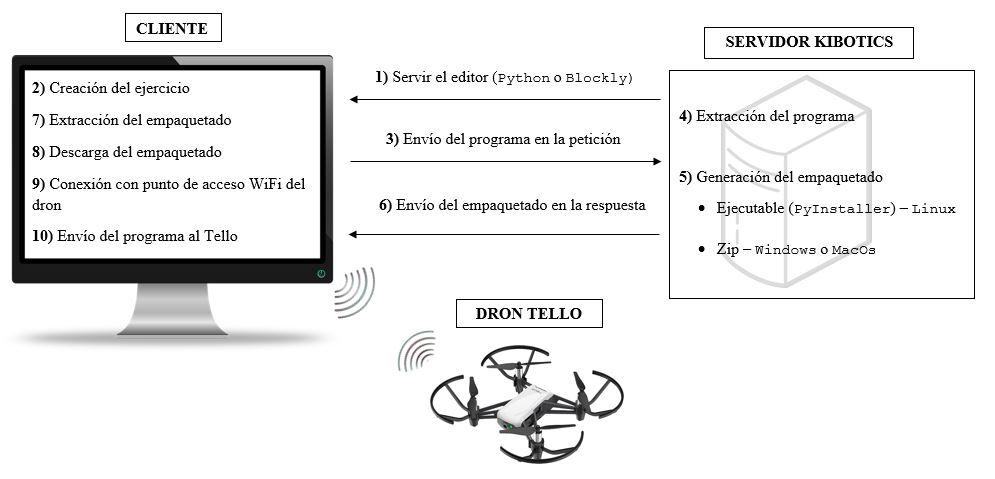
\includegraphics[width=1\textwidth]{images/infraestructura_tello.png}
  \caption{Arquitectura del desarrollo para el Tello}
  \label{Arquitectura del desarrollo para el Tello}
\end{figure}
\\
A continuación hablaremos en detalle sobre los pasos necesarios para conseguir la integración del Tello en Kibotics en los sistemas operativos Linux, Windows y MacOs.

\section{Lado cliente}

En la parrilla de Kibotics se encuentran dos unidades dedicadas al dron Tello , una dedicada a su programación utilizando Python y otra con Blockly. En la unidad se encuentra una sección que proporciona información sobre los requisitos para este robot y cómo utilizarlo. 
\\
\\
Para el Mbot no se requería ninguna instalación y, además, el proceso de envío del programa era el mismo para los diferentes sistemas operativos. En el caso del Tello, existen peculiaridades para los diferentes sistemas operativos al no tener control sobre la controladora que posee el robot y al necesitar un proxy intermediario. Aunque en el robot no es necesario instalar nada, si que se necesitarán unos requisitos previos para los ordenadores que sean Windows y MacOs.

\subsection{Preparación del anfitrión}

Para MacOs y Windows, es indispensable que el usuario tenga instalado Python en su versión 2.7 y los drivers necesarios para el uso del Tello. La empresa Dji-sdk posee un repositorio en GitHub (https://github.com/dji-sdk/Tello-Python) en el que se facilitan instaladores para su uso en los diferentes sistemas operativos. Por lo que el usuario tendría que instalar estos requisitos. Aunque para el caso de MacOs, cuando se carga el programa a el robot si no dispone de estos requisitos los instalará (sección 5.3.6).
\\
\\
En Linux, sin embargo, no es necesaria ninguna instalación previa para poder utilizar este dron. Esto es gracias a PyInstaller, una librería de Python, y a que el servidor de Kibotics se encuentra en una máquina Linux. En las próximas secciones se profundizará en este aspecto.

\subsection{Editor}

En la unidades se tiene también un editor (Python o Blockly ), adaptado a la porgramación del Tello, donde el usuario podrá realizar su programa. El aspecto es similar al los utilizados para el Mbot. 
\\
\\
Una vez que el usuario ha desarrollado el programa, debería pulsar el botín azul llamado “Ejecutar en Tello” (Figura 5.2) para iniciar el proceso de envío, que variaría dependiendo del sistema operativo utilizado.
\\
\begin{figure}[h!]
  \centering
    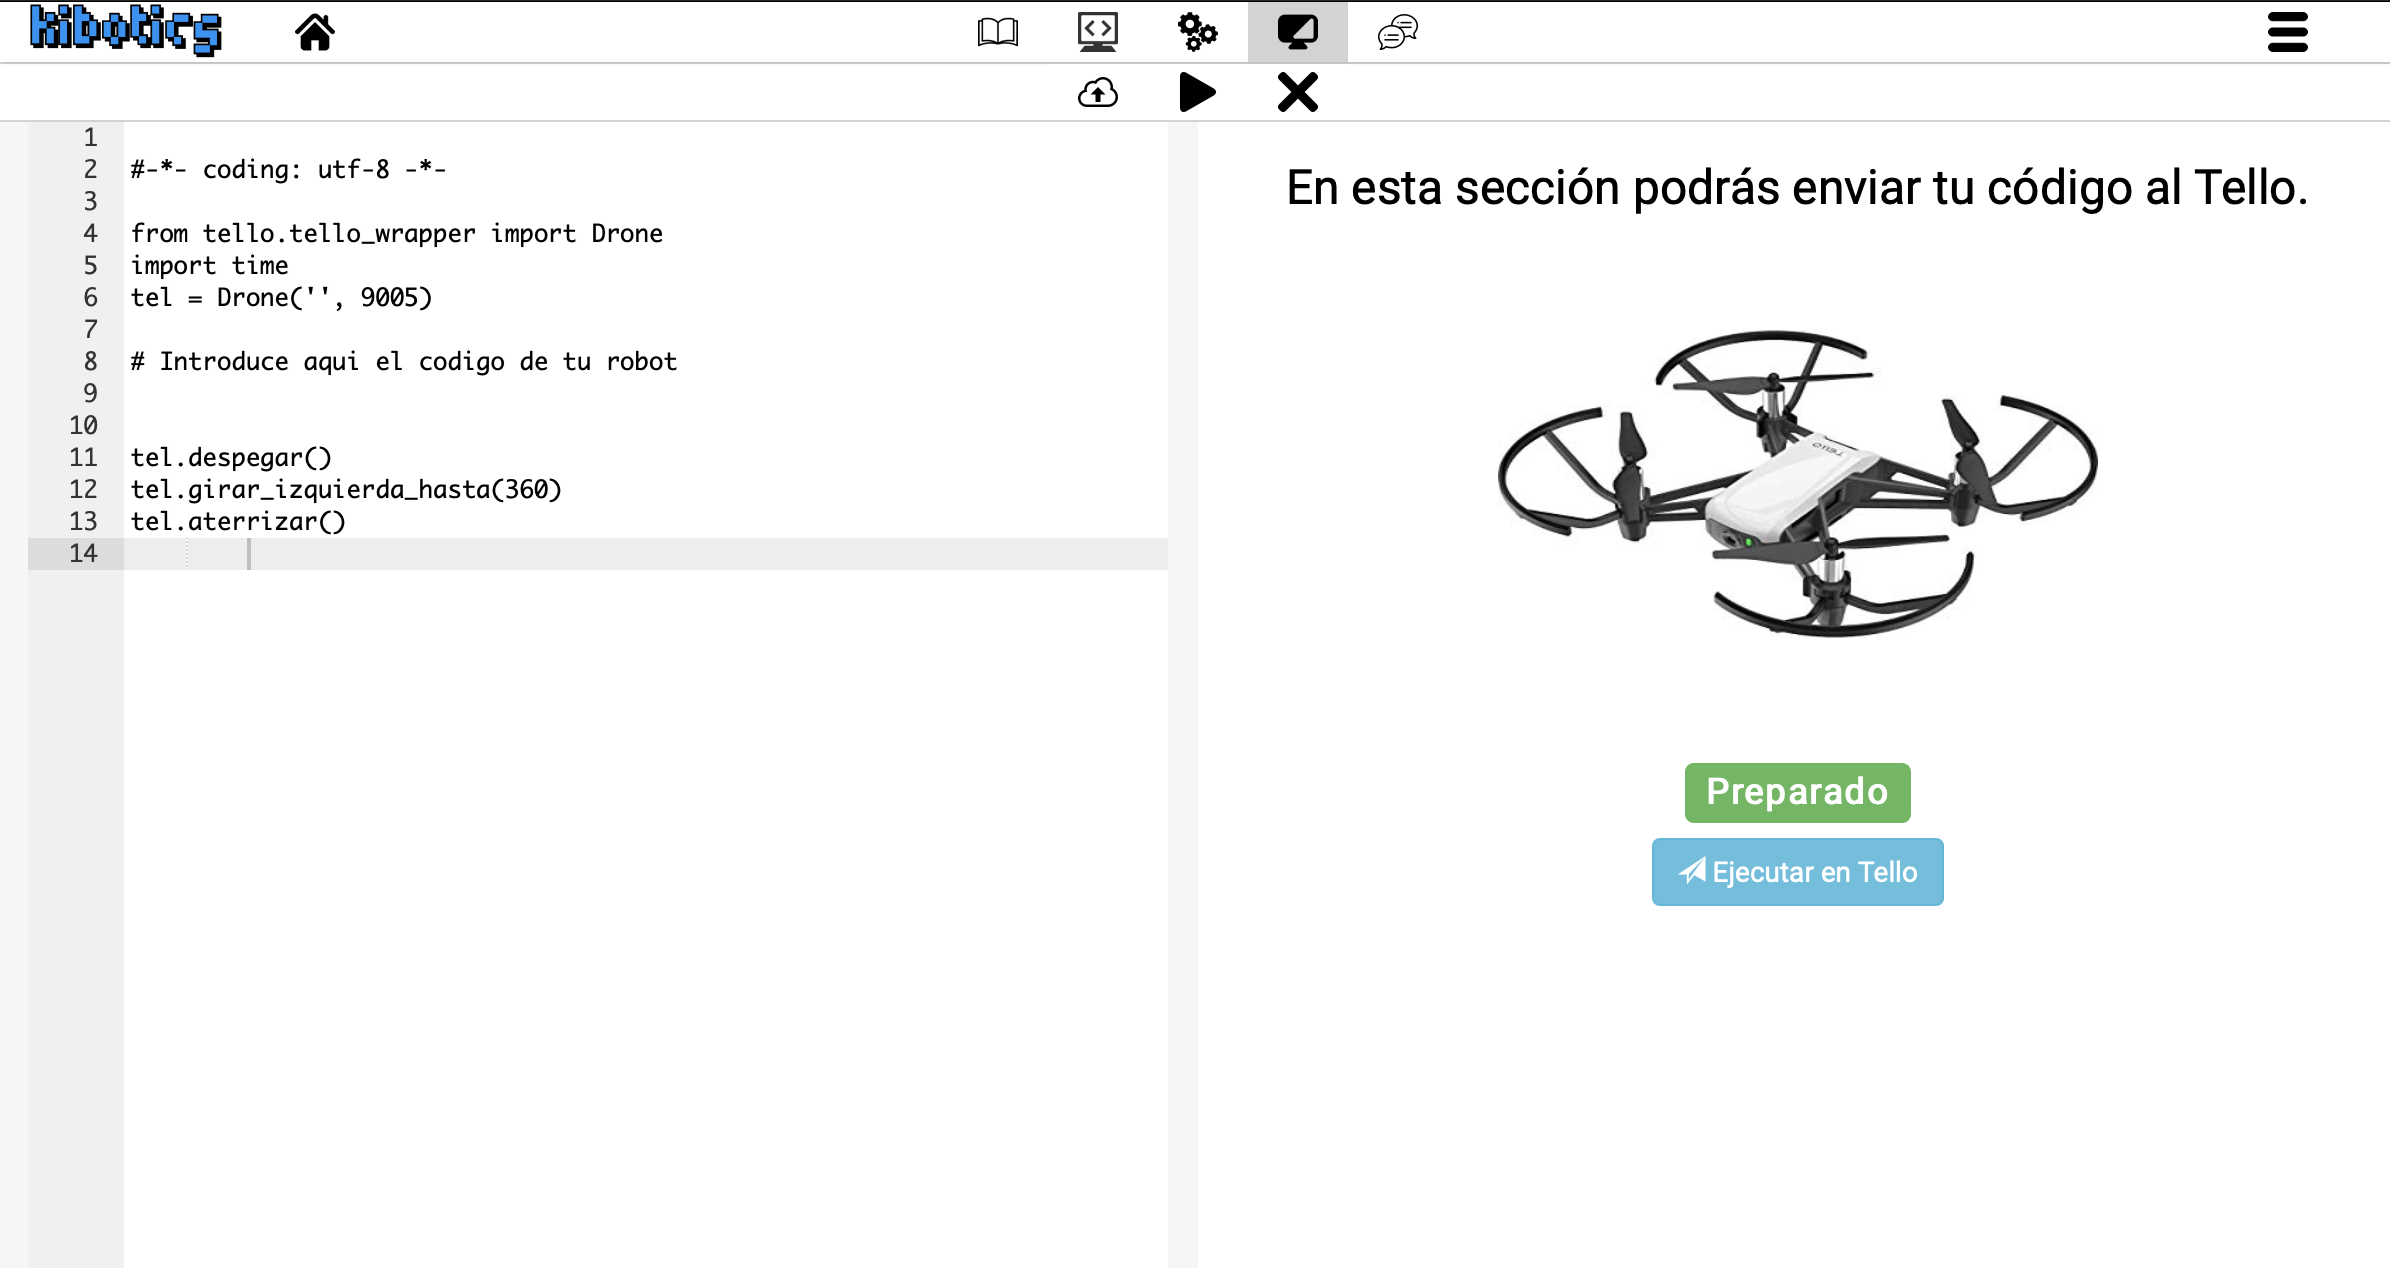
\includegraphics[width=0.9\textwidth]{images/editor_tello.png}
  \caption{Editor para programar el dron Tello en Python}
  \label{Editor para programar el dron Tello en Python}
\end{figure}


\subsection{Envío del código fuente al servidor}

Una vez iniciado el proceso de envío, el primer paso es enviar el código escrito por el usuario a el servidor de Kibotics, para generar el ejecutable que permita enviar el programa al Tello. 
\\
\\
Se extrae el código escrito en el editor y se envía desde el navegador al servidor en un query parameter de una petición GET (Fragmento 5.1).
\\
\begin{lstlisting}[frame=single,breaklines=true, label=Envio del programa desde el navegador al servidor", caption=Envio del programa desde el navegador al servidor,captionpos=b]
   
   function send_code_tello() {
      var editor = ace.edit("ace");
      let code = editor.getValue();
      console.log(code);
      const message = {
         method: "GET"
       };
       var = url = '/get_code_to_tello?python_code=' + JSON.stringify(code);
       fetch(url, message)
             . . . . .
  }
\end{lstlisting}




\subsection{Recepción del ejecutable}

El navegador queda a la espera de recibir la respuesta a la petición que envió al servidor. Y tras obtener esta respuesta, extraerá un ejecutable en el caso de que se use una máquina Linux, o un fichero comprimido en el caso de usar Windows o MacOS, que preparó el servidor y que permitirá realizar la carga del programa.  Posteriormente, el fichero extraído se descargará en el ordenador de usuario.
\\
\begin{lstlisting}[frame=single,breaklines=true, label=Extracción empaquetado y descarga, caption=Extracción empaquetado y descarga,  captionpos=b]
   . . .
   
   var = url = '/get_code_to_tello?python_code=' + JSON.stringify(code);
   fetch(url, message)
      .then(response => {
         ld.style.display = "none";
         if (response.ok) {
            download_executable(response);
         } else {
            console.error("Bad Response");
         }
      })
     .catch(err => console.error(err));
   }
   
   function downloadExecutable(response) {
      response.blob().then(blob => {
         var down = document.createElement("down");
         document.body.appendChild(down);
         down.style = "display: none";
         url = window.URL.createObjectURL(blob);
         down.href = url;
         down.download = 'tello_code';
         down.click();
         window.URL.revokeObjectURL(url)
      })
   }
\end{lstlisting}

\subsection{Conexíón con el drone}

Para poder enviar el programa el Tello, necesitamos estar conectados con él. El dron, una vez encendido, emite un punto de acceso WiFi, que tendrá el nombre Tello seguido de un número (Figura 5.5 ), al que se tiene que conectar el usuario para posteriormente cargarle el programa. Necesitamos de esta pasarela para comunicarnos con él.
\\
\begin{figure}[h!]
	\centering
    	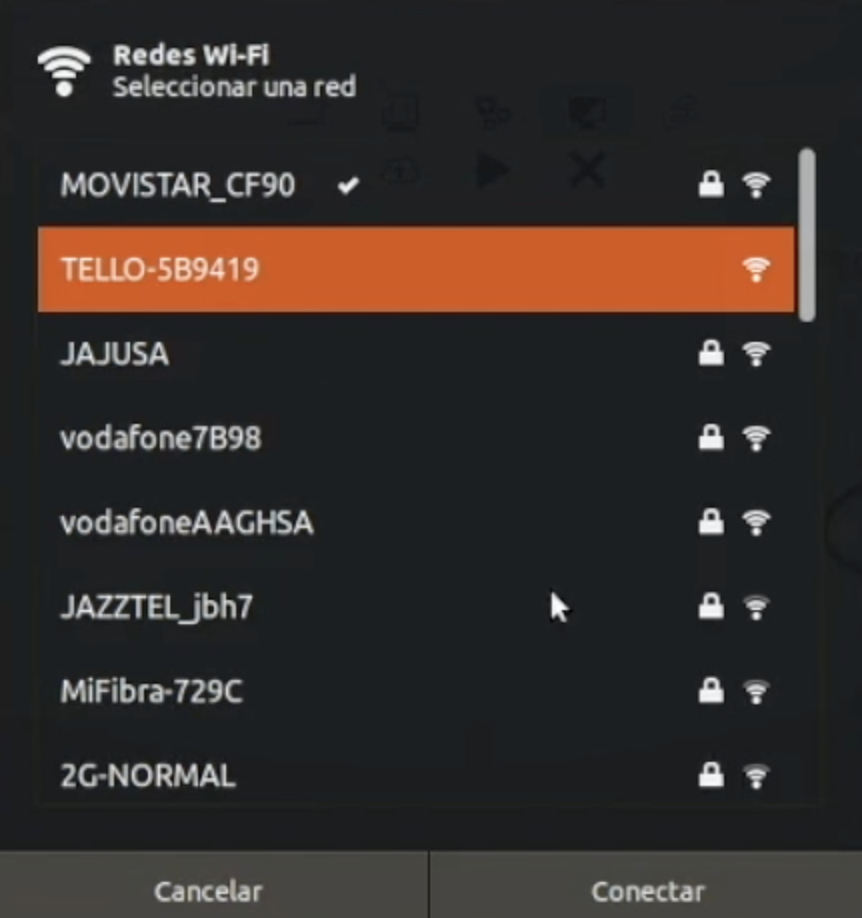
\includegraphics[width=0.4\textwidth]{images/seleccionar_wifi_tello.png}
  	\caption{Conectarse al punto de acceso WiFi emitido por el dron}
  	\label{Conectarse al punto de acceso WiFi emitido por el dron}
\end{figure}


\subsection{Ejecución}


El fichero descargado en el ordenador permitirá enviar el programa al Tello, como este fichero es diferente para cada uno de los sistemas operativos, el proceso que hay que seguir para ejecutarlo no es el mismo. A continuación se describe cual es el proceso de ejecución para cada uno de los sistemas operativos:
\begin{itemize}
	\item \textbf{Linux.} 
		\begin{enumerate}
			\item Se descargará un ejecutable.
			\item Dirigirse al directorio donde se descargo, darle permisos de ejecución y ejecutarlo (Fragmento 5.3).
			\\
			\begin{lstlisting}[frame=single,breaklines=true, label=Comandos para ejecución del envío en MacOs, caption=Comandos para ejecución del envío en MacOs,  captionpos=b]
		chmod +x send_code.sh &&
		./send_code.sh
			\end{lstlisting}
		\end{enumerate}
	\item \textbf{Windows.} 
		\begin{enumerate}
			\item Se descargará un fichero comprimido.
			\item Descomprimir el fichero y dirigirse a  directorio extraído.
			\\
			\begin{figure}[h!]
 			 	\centering
    				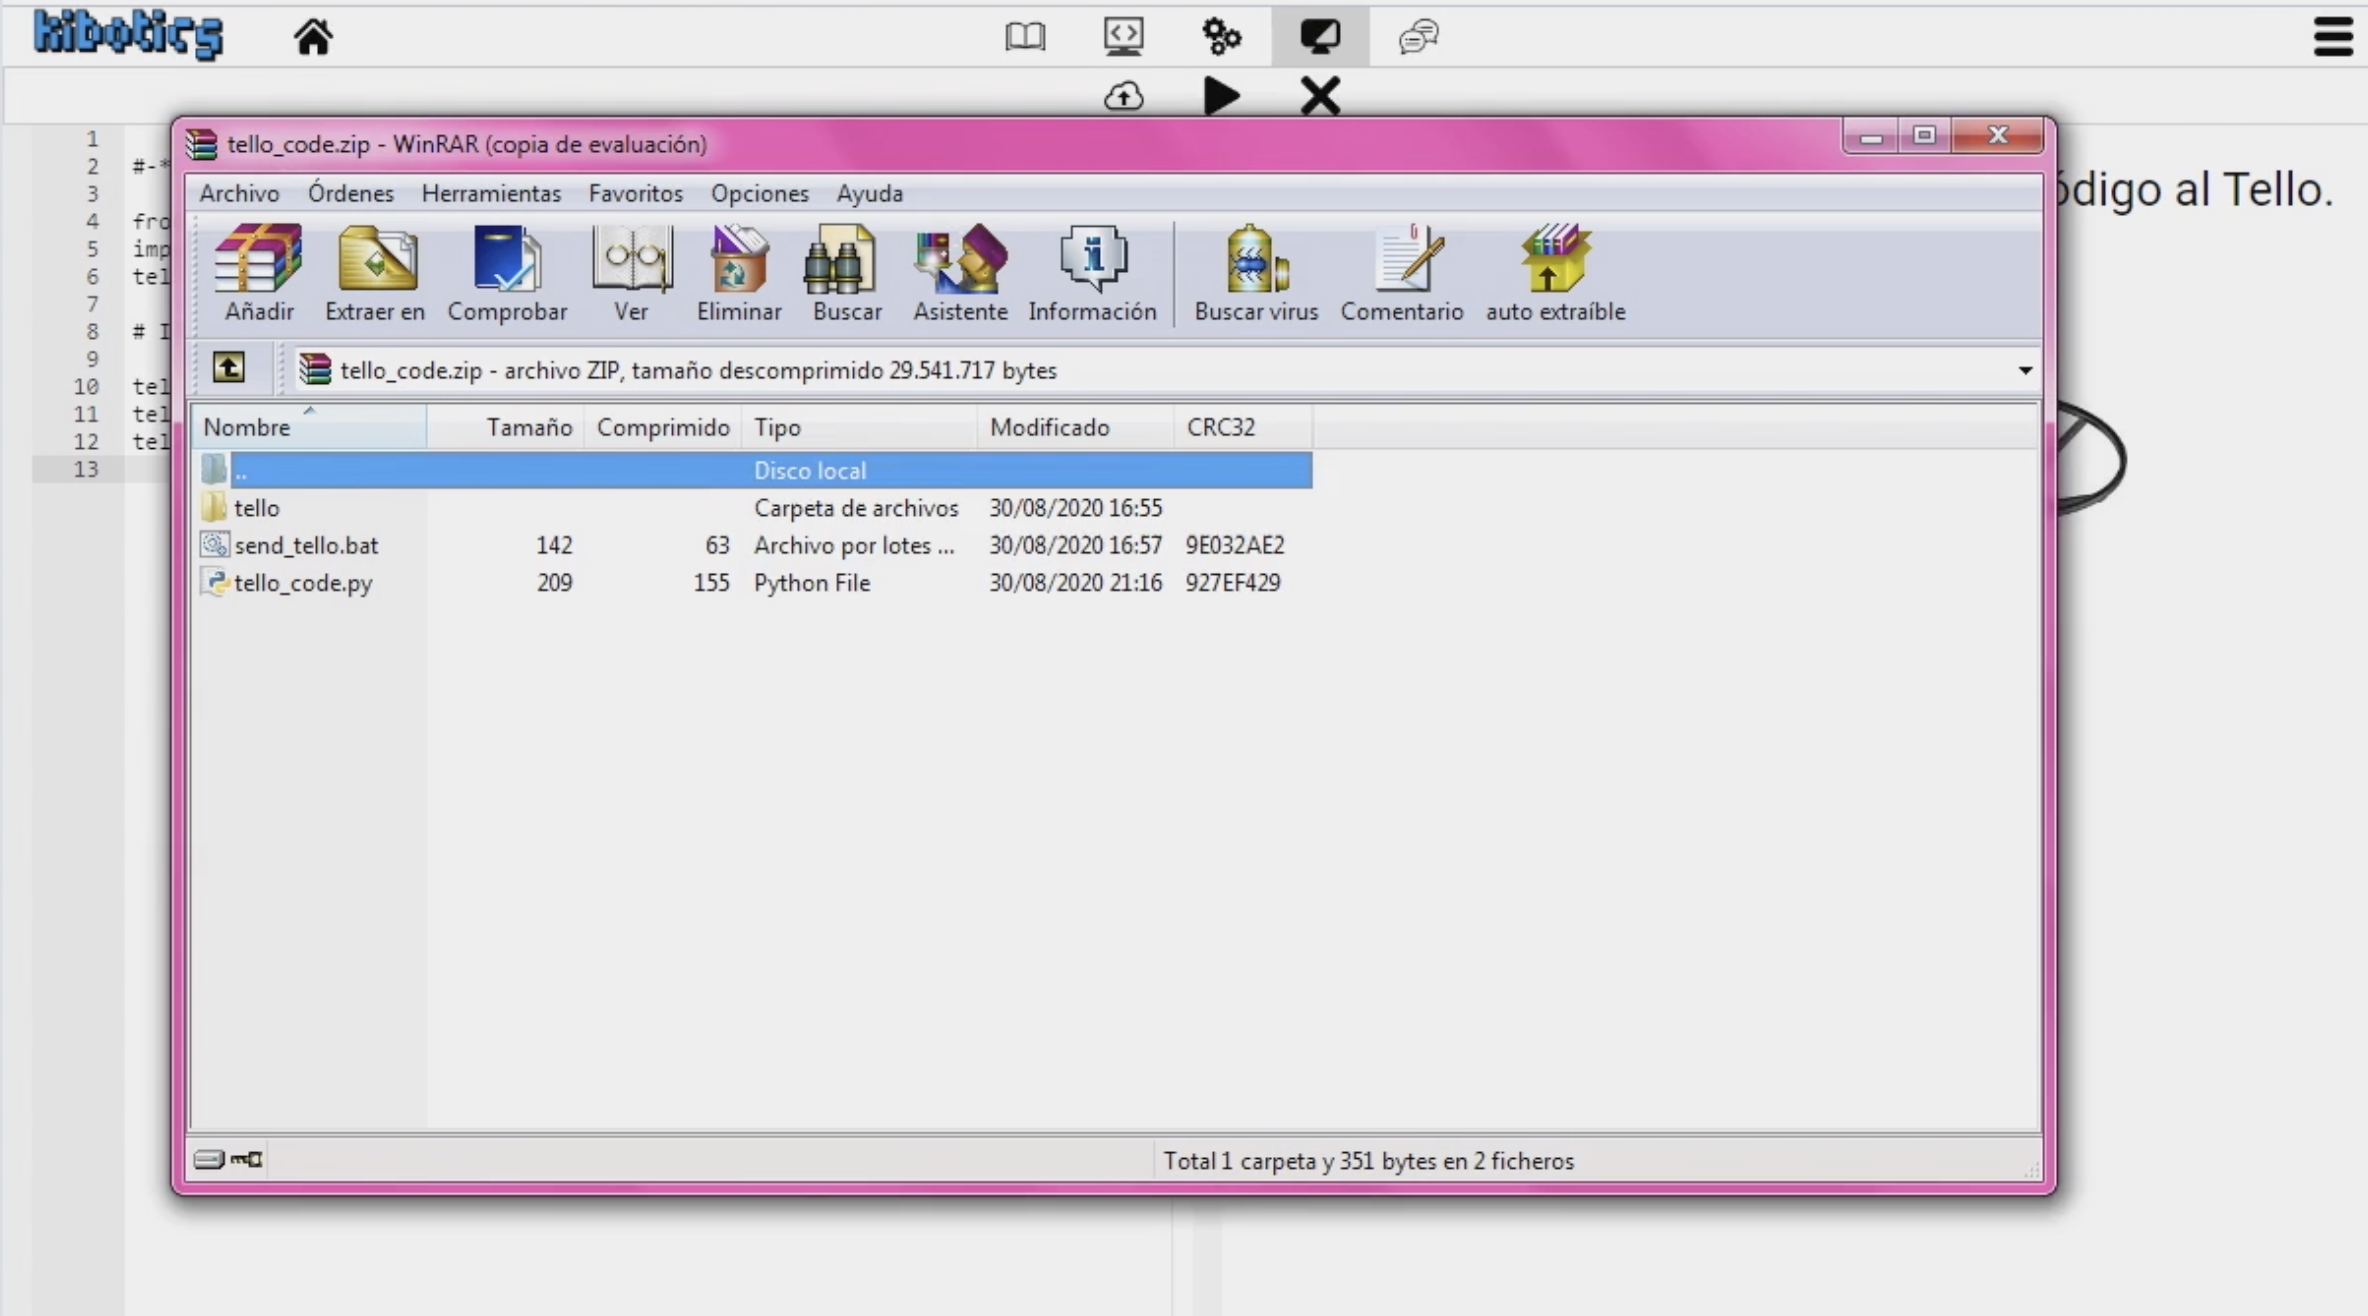
\includegraphics[width=1\textwidth]{images/descarga_windows_tello.png}
  				\caption{Descompresión en Windows}
  				\label{Descompresión en Windows}
			\end{figure}
			\item Haciendo doble “click” en el ejecutable send\_tello.bat, el programa será enviado al Tello.
		\end{enumerate}
	\item \textbf{MacOs.}
		\begin{enumerate}
			\item Se descargará un fichero comprimido.
			\item Descomprimir el fichero y dirigirse a  directorio extraído.
			\item Dentro del directorio se encuentra un fichero ejecutable llamado "send\_code.sh", al que se tendrá que dar permisos de ejecución y, posteriormente, ejecutarlo para enviar el programa al dron (Fragmento 5.4).			
			\\
			\begin{lstlisting}[frame=single,breaklines=true, label=Comandos para ejecución del envío en MacOs, caption=Comandos para ejecución del envío en MacOs,  captionpos=b]
		chmod +x send_code.sh &&
		./send_code.sh
			\end{lstlisting}
		\end{enumerate}

		El ejecutable que se utiliza en MacOS para el envío (send\_code.sh), con el objetivo de facilitar las instalaciones requeridas para el Tello, instalará todas las dependencias necesarias en el caso de que no se tengan en el ordenador.
		\\
\begin{lstlisting}[frame=single,breaklines=true, label=Ejecutable de envio para MacOs, caption=Ejecutable de envio para MacOs,  captionpos=b]
   #!/bin/bash

   ######### Requirements #########

   env=~/.virtualenvs/tello-env
   if [ -d $env ];
   then
      source ~/.virtualenvs/tello-env/bin/activate
   else
      if ! type "pip" > /dev/null; then
         sudo easy_install pip
       fi
       if ! type "brew" > /dev/null; then
          /usr/bin/ruby -e "$(curl -fsSL https://raw.githubusercontent.com/Homebrew/install/master/install)"  
          brew update
       fi
       sudo brew install cmake
       sudo brew install boost
       sudo brew install boost-python
       sudo brew install ffmpeg
       sudo brew install tcl-tk
    
       mkdir ~/.virtualenvs
       pip install virtualenv
       virtualenv ~/.virtualenvs/tello-env --python=python2.7
       source ~/.virtualenvs/tello-env/bin/activate
       pip install SimpleWebSocketServer
       pip install numpy
       pip install matplotlib
       pip install opencv-python==3.1.0.1
   fi

   echo "################################"
   echo "### Sending program to tello ###"
   echo "################################"
   python tello_code.py
   echo "Program finished"
   deactivate
\end{lstlisting}

\end{itemize}



\section{Lado servidor}

Como ocurría en el Mbot, el servidor de Kibotics, además de ser el responsable de servir las páginas, también es el encargado de adaptar el código que ha escrito el usuario para que el programa pueda ser enviado al dron. 
\\
\\
En este caso, la adaptación consistirá en realizar un empaquetado que será devuelvo a el navegador. En los siguientes apartados se describen los pasos seguidos para conseguirlo.

\subsection{Recepción del código fuente}

Una vez que el usuario ha realizado el programa y se ha iniciado el proceso de envió, el navegador envía el código escrito por el usuario al servidor. Este extrae dicho código del query parameter de la petición recibida (Fragmento 5.5). 
\\
\begin{lstlisting}[frame=single,breaklines=true, label=Extracción programa en el servidor, caption=Extracción programa en el servidor, captionpos=b]
   def get_code_to_tello(request):
      . . . .
      python_code = json.loads(request.GET.get('python_code', None))
      . . . .

\end{lstlisting}


\subsection{Empaquetado}

El dron Tello entiende el lenguaje Python, y como el código extraído ya se encuentra escrito en este lenguaje, no será necesaria realizar ninguna conversión. Por lo tanto, una vez extraído el código se procede a su empaquetado, que será diferente en función del sistema operativo utilizado por el usuario.
\\
\begin{itemize}
	\item \textit{\textbf{Linux}}. El empaquetado consistirá en realizar un ejecutable que contenga todas las dependencias necesarias para el envío. Esto es posible gracias a una librería de Python llamada PyInstaller, un módulo que permite empaquetar ficheros Python, generando así un ejecutable e incluyendo dentro del propio ejecutable el intérprete de Python. PyInstaller no permite una compilación cruzada, es decir, si este empaquetado se realiza en una máquina Linux, el ejecutable solo podrá utilizarse en una máquina Linux. Debido a esto, la integración para el dron Tello varía según el sistema operativo; como el servidor de Kibotics está alojado en una máquina Linux, solo los usuarios de Linux se beneficiarán de esta utilidad.
\begin{lstlisting}[frame=single,breaklines=true, label=Creación ejecutable con PyInstaller, caption=Creación ejecutable con PyInstaller,  captionpos=b]
   def create_executable_with_pyinstaller(exercice_path):
    		      
   	call(". kibotics-drivers/tello/tello_env/bin/activate; pyinstaller -F --distpath " +
      	exercice_path + "dist --workpath " + exercice_path + "build --specpath " + exercice_path + " --clean " + exercice_path +
      	"tello_code.py", shell=True)
      . . . 
\end{lstlisting}
	
	
	\item \textit{\textbf{Windows y MacOs}}. El proceso es similar en ambos, pero diferente al caso anterior. Se empaqueta el programa con el directorio que engloba todas las librerías y las dependencias necesarias y que, además, contiene el ejecutable .bat (en Windows) o .sh (en MacOS) que se encargará del envío (Fragmento 5.7). La única diferencia entre ambos, es que al necesitar dependencias especificas por sistema operativo, se utilizan directorios diferentes en el empaquetado.
	\\
\begin{lstlisting}[frame=single,breaklines=true, label=Creación empaquetado en Windows y MacOs, caption=Creación empaquetado y respuesta en Windows y MacOs,  captionpos=b]
   if operative_system == 'Mac':
        shutil.move(exercise_dir + "tello_code.py", os.getcwd() + "/kibotics-drivers/tello/MacOs")
        shutil.make_archive('output-tello-mac', 'zip', os.getcwd() + "/kibotics-drivers/tello/MacOs")

    elif operative_system == 'Windows':
        shutil.move(exercise_dir + "tello_code.py", os.getcwd() + "/kibotics-drivers/tello/Windows")
        shutil.make_archive('output-tello-windows', 'zip', os.getcwd() + "/kibotics-drivers/tello/Windows")

\end{lstlisting}	

\end{itemize}


\subsection{Envío del ejecutable}

Una vez generado el empaquetado, ejecutable en Linux y fichero comprimido en MacOs y Windows, se devuelve al navegador en la respuesta a la petición que envió. Esto permitirá que sea descargado en el ordenador del usuario y pueda ejecutarlo, consiguiendo así el proceso de envió del programa al dron Tello.
	\\
\begin{lstlisting}[frame=single,breaklines=true, label=Respuesta a la petición para Linux, caption=Respuesta a la petición para Linux,  captionpos=b]
   create_executable_with_pyinstaller(exercice_path)
   response = FileResponse(open(exercice_path + "dist/tello_code", 'rb'), content_type='application/octet-stream')
   shutil.rmtree(exercise_dir + "dist/")
   shutil.rmtree(exercise_dir + "build/")
   os.remove(exercise_dir + "tello_code.spec")
\end{lstlisting}
\begin{lstlisting}[frame=single,breaklines=true, label=Respuesta con empaquetado en Windows y MacOs, caption=Creación empaquetado y respuesta en Windows y MacOs,  captionpos=b]
   if operative_system == 'Mac':
        . . . 
        with open('output-tello-mac.zip', 'rb') as f:
            response = HttpResponse(f, content_type=guess_type('output-tello-mac.zip')[0])
            response['Content-Length'] = len(response.content)
            os.remove('output-tello-mac.zip')

    elif operative_system == 'Windows':
        . . .
        shutil.move(exercise_dir + "tello_code.py", os.getcwd() + "/kibotics-drivers/tello/Windows")
        shutil.make_archive('output-tello-windows', 'zip', os.getcwd() + "/kibotics-drivers/tello/Windows")
        os.remove(os.getcwd() + "/kibotics-drivers/tello/Windows/tello_code.py")
        with open('output-tello-windows.zip', 'rb') as f:
            response = HttpResponse(f, content_type=guess_type('output-tello-windows.zip')[0])
            response['Content-Length'] = len(response.content)
            os.remove('output-tello-windows.zip')
\end{lstlisting}	

\section{Validación experimental}

La tecnología utilizada en este caso es distinta a la del Mbot debido a las diferencias en las controladoras del robot; con la placa mCore, el control sobre ella es mayor, mientras que en la que utiliza el Tello no tenemos ningún control.
\\
\\
Otro aspecto importante es que para el envío del programa al Tello se necesita una pasarela, es decir, para poder comunicarnos con él necesitamos conectarnos al punto de acceso WiFi que emite el dron, por lo que no es posible un envío directo desde el navegador, algo que sí se podía hacer en el Mbot con Web Serial.
\\
\\
Por otro lado, la tecnología PyInstaller permite que el usuario interaccione con el dron sin necesidad de instalar previamente nada, y también simplifica el envío al lanzar el ejecutable descargado. El problema que surge es que, con la restricción de compilación cruzada, este proceso solo puede ser factible para Linux, ya que el servidor de Kibotics, que es el encargado de preparar el ejecutable, está alojado en una máquina Linux.
\\
\\
Para Windows y MacOs la situación cambia completamente. El usuario sí necesita tener instalado en su ordenador el intérprete Python2.7 y los drivers para poder usar el Tello, aunque en MacOs el ejecutable de envío será el que lo instale si el usuario no lo tiene, facilitando, por tanto, su uso. Además, el envío del programa no es tan directo, ya que en primer lugar hay que descomprimir el fichero descargado, que tiene las dependencias necesarias para el envío y, después, se lanza el ejecutable.
\\ 
\\
Para su experimentación se ha probado en diferentes sistemas operativos (\textit{Ubuntu 18.04}, \textit{Ubuntu 16.04}, \textit{Windows 10}, \textit{Windows 7}, \textit{MacOs Catalina Versión 10.15.6}, \textit{MacOs Mojave Versión 10.14.6}) y navegadores (\textit{Safari Versión 14.0}, \textit{Google Chrome Versión 85.0}, \textit{Firefox Versión 68.9}), verificando así que la integración permite ser multiplataforma.
\\
\\
Por último, en lo siguientes punteros a vídeos, se muestra un ejemplo de realización y envió de un programa al dron Tello, para los principales sistemas operativos, desde la plataforma de Kibotics.
\begin{itemize}
	\item En Linux:  \textit{https://www.youtube.com/watch?v=b\_msB5vBw4A\&t=8s}
	\item En Windows:  \textit{https://youtu.be/vfRo9dGXbBw}
	\item En MacOs: \textit{https://youtu.be/SAa1XO8Cp\_o}
\end{itemize}

\begin{figure}[h!]
  \centering
    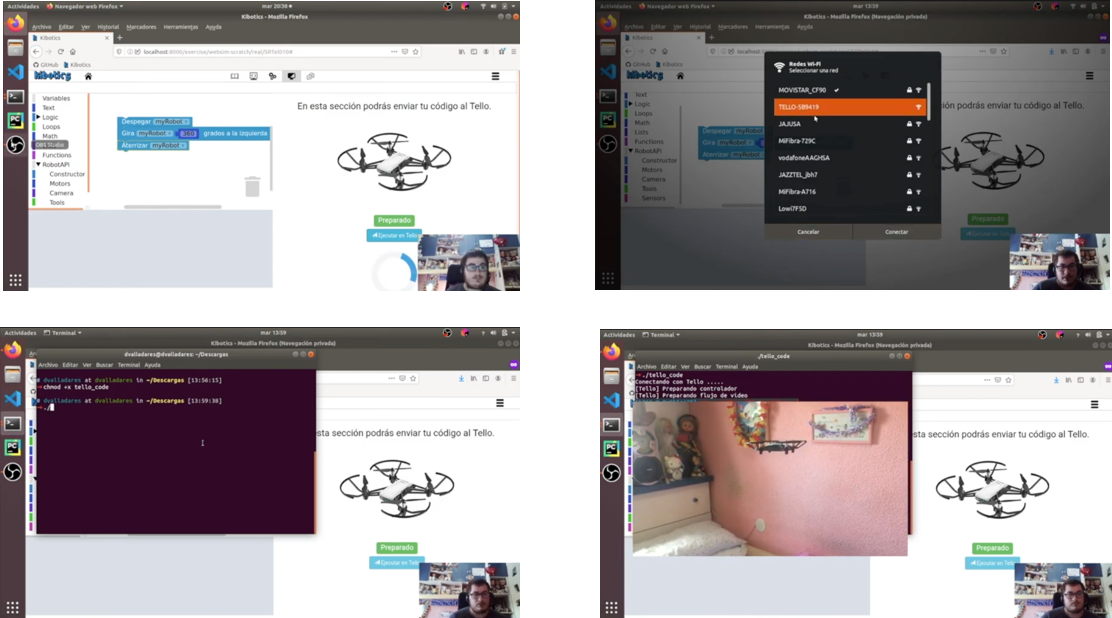
\includegraphics[width=1\textwidth]{images/fotogramas_tello.png}
  \caption{Fotogramas del vídeo de ejemplo de realización de un programa para el Tello en Linux}
  \label{Fotogramas del vídeo de ejemplo de realización de un programa para el Tello en Linux}
\end{figure}


%###############################################################################
%###################### GoPiGo ##################################################
%###############################################################################

\chapter{Integracion GoPiGo3 en Kibotics}

Al igual que en los capítulos mostraremos cuál ha sido el desarrollo realizado para llevar, en este caso, el robot GoPiGo3 a la plataforma Kibotics, lo que permitirá su programación.

\section{Robot GoPiGo3}

GoPiGo es un proyecto llevado a cabo por Dexter Industries, que pretende integrar la Raspberry Pi en los robots, dotándoles así de una mayor inteligencia y flexibilidad. Actualmente se encuentra en su versión GoPiGo3, que consiste en un kit robótico con forma de vehículo (Figura 6.1).
\\
\\
Entre las características del hardware del GoPiGo3 destaca su cuerpo, que consiste en un acrílico grueso. Requiere un voltaje de entre 7-12V, con una batería a pilas. Dispone de una placa llamada “GoPiGo3", que se conecta a la Raspberry Pi. La comunicación con la controladora se produce a través de la interfaz SPI (Serial Peripheral Interface). Incluye dos motores para conectarlo a las ruedas, las cuales tienen 66,5 mm de diámetro. También dispone de codificadores electrónicos, que se conectan a los motores para mejorar la movilidad. Respecto a las interfaces externas, destacan los dos puertos I2C (Inter-Integrated Circuit) y los puertos seriales que están acoplados a los pines de la Raspberry Pi (Dexter Industries, 2020).
\\
\begin{figure}[h!]
  \centering
    \includegraphics[width=1\textwidth]{images/partes_GoPiGo.png}
  \caption{Hardware GoPiGo3}
  \label{Hardware GoPiGo3}
\end{figure}
\\
Dexter Industries también ha desarrollado DexterOS, que incluye el software necesario para que la Raspberry Pi funcione con GoPiGo3 (Dexter Industries, 2020). DexterOS se distribuye mediante una SD (Secure Digital) de 8GB que se inserta en la ranura de la Raspberry Pi. Este software emite una señal WiFi que, una vez que el usuario se ha conectado a ese punto de acceso, al acceder al navegador se obtiene una web que permite interactuar con el robot sin necesidad de realizar ninguna descarga previa en el ordenador (Figura 6.2).
\\
\begin{figure}[h!]
  \centering
    \includegraphics[width=1\textwidth]{images/software_GoPiGo.png}
  \caption{Sotfware para GoPiGo3}
  \label{Sotfware para GoPiGo3}
\end{figure}
\\
Esta web dispone de cuatro módulos. El primero incluye lecciones integradas para aprender a programar el GoPiGo3 y algunos conceptos sobre los sensores de los que dispone. Otro módulo ofrece la posibilidad de conducir el GoPiGo3 de forma remota. Los otros dos módulos sirven como editores para programar el robot, de manera que uno de ellos permite programarlo mediante un lenguaje basado en bloques llamado “Bloxter” (Figura 6.3), muy similar a Blockly y diseñado por la propia empresa, mientras que el otro sirve para programarlo en Python (Dexter Industries, 2020). También han creado librerías que facilitan su programación para este lenguaje (una de ellas se llama “EasyGoPiGo3”)
\\
\begin{figure}[h!]
  \centering
    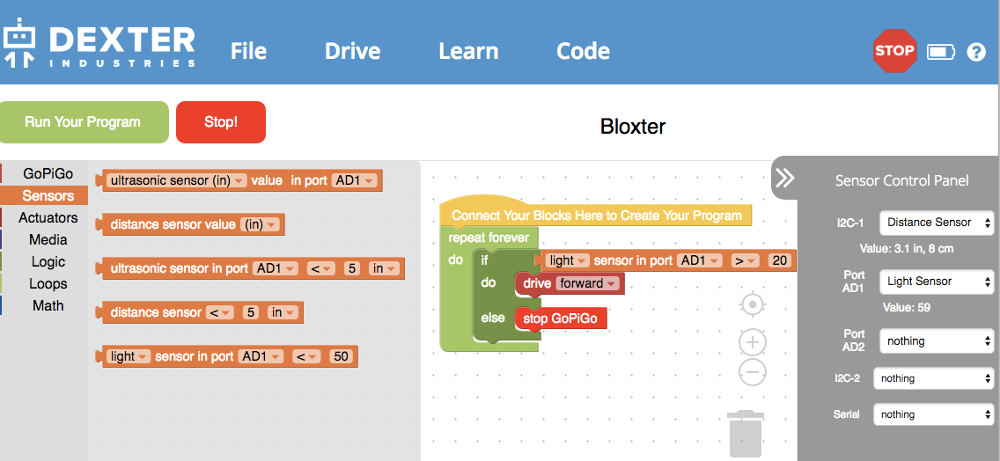
\includegraphics[width=1\textwidth]{images/editor_bloxter.png}
  \caption{Editor Bloxter}
  \label{Editor Bloxter}
\end{figure}

\section{Diseño}

La figura 6.4 muestra el diseño seguido para llevar el GoPiGo3 a la plataforma Kibotics. En comparación con el diseño para los dos robots anteriores, en este caso se utiliza un servidor adicional que permitirá la recepción del programa en el robot.
\\
\begin{figure}[h!]
  \centering
    \includegraphics[width=1\textwidth]{images/arquitectura_GoPiGo.png}
  \caption{Diseño para la integración del GoPiGo3}
  \label{Diseño para la integración del GoPiGo3}
\end{figure}
\\
En los siguientes capítulos se profundizará en este diseño y en las interacciones necesarias entre el cliente, el servidor de Kibotics y el servidor de la Raspberry Pi, que permitirá programar al GoPiGo3.

\section{Lado Cliente}

En la parrilla de unidades de Kibotics, se puede encontrar una unidad dedicada al GoPiGo3 para Python. Actualmente solo está disponible para este lenguaje.
\\
\\
En una de secciones de la unidad se proporciona información al usuario sobre cómo realizar el envío, así como de las instalaciones que deben realizar. En este caso solo tiene que hacer instalaciones en la Raspberry Pi del robot, ya que en el ordenador del anfitrión no es necesaria ninguna instalación. En el fragmento 6.1 se muestran los detalles de cómo se ha diseñado esta sección.
%\\
%\begin{figure}[h!]
%  \centering
%    \includegraphics[width=1\textwidth]{images/info_GoPiGo.png}
%  \caption{Página de información del GoPiGo3}
%  \label{Página de información del GoPiGo3}
%\end{figure}
\\
\begin{lstlisting}[frame=single,breaklines=true, label=Página de información del GoPiGo3, caption=Página de información del GoPiGo3,  captionpos=b]
<html>
<head>
<meta charset='UTF-8'><meta name='viewport' content='width=device-width initial-scale=1'>
<title>GoPiGo3</title></head>
<body><h1>GoPiGo3 example</h1>
<p>Podras realizar tu programa para enviarselo al GoPiGo.</p>
<p><img src="" width=200px></p>

<h2>1 - Instalacion</h2>
<ul>
 <li type="circle">
  <h4>   <b>En la Raspberry Pi 3 del GoPiGo3:</b> </h4>
   <ol start='1' >
    <li>
     Descargar el siguiente fichero comprimido => <a href="" target="_blank">Intalador</a>
    </li>
    <li>
     Descomprimir el Zip descargado y situarlo en el directorio /home/pi/
    </li>
    <li>
     Ir al directorio e instalar los drivers necesario, para ello abrir un terminal y ejecutar
    </li>
    <ol start='1' >
     <li>
      <code>chmod +x instalar_drivers_GoPiGo.sh</code>
     </li>
     <li>
      <code>./instalar_drivers_GoPiGo.sh</code>
     </li>
    </ol>
    <li>
     Agregar la instruccion que permite levantar siempre el servidor al encenderse la Raspberry, para ello dirigirse al directorio y abrir un terminal:</li> 
     <ol start='1' >
      <li>
       Ejecutar => <code>chmod +x iniciar_servidor_GoPiGo.sh</code>
      </li> 
      <li>
       Abrir el servicio cron => <code>crontabl -e</code>
      </li> 
      <li>
       Agregar la tarea <code> @reboot /home/pi/configuracion_GoPiGo/iniciar_servidor_GoPiGo.sh &</code>
      </li> 
     </ol>
   </ol>
   </li>
   <li type="circle">
    <h4>   <b>En el ordenador MacOs/Linux/Windows:</b> </h4>
     <p>No es necesaria ningun tipo de instalacion adicional para el funcionamiento.</p>
    </li>
</ul>

<h2>2 - Ejecucion</h2>
<ol start='' >
 <li>
  Realice su programa
 </li>
  <li>
   Eciende el GoPiGo y asegurate de que esta conectado a el WiFi. 
  </li>
  <li>
   Pulse en <b>Enviar</b>, si todo ha ido bien se cargara el programa en el GoPiGo3. 
  </li>
</ol>
</body>
</html>
\end{lstlisting}

\subsection{Editor}

Para escribir un programa y enviarlo al robot desde el lado del cliente, otra sección de la unidad proporciona un editor donde el usuario podrá escribir su programa utilizando el lenguaje Python. En el editor se importa la librería “EasyGoPiGo3” (Dexter Industries, 2018), que proporciona una Api para interactuar con los sensores y actuadores del robot (Figura 6.5).
\\
\begin{figure}[h!]
  \centering
    \includegraphics[width=1\textwidth]{images/editor_GoPiGo.png}
  \caption{Editor python para el GoPiGo3}
  \label{Editor python para el GoPiGo3}
\end{figure}
\\

\subsection{Envío del código al servidor del Robot}

Una vez que el usuario ha escrito el programa deseado, deberá pulsar el botón “Enviar” que puede verse en la figura 6.5, el cual desencadenará todo el proceso de envío. En el fragmento 6.2 se muestra cuál es el código HTML que permite iniciar este proceso.
\\
\begin{lstlisting}[frame=single,breaklines=true, label=Sección para el envió, caption=Sección para el envió,  captionpos=b]
<center><h3>En esta seccion podras enviar tu codigo  al GoPiGo3.</h3></center>

<div class="text-center">
 <img class="text-center" src="{{ exercise.language }}/{{ exercise.exercise_id }}/img/GoPiGo3.png" width="300px" height="250px">
</div>

<div id="text" class="text-center">
 <h3><span id="proxy_state" class="label label-success">Conexion con proxy</span></h3>
  <button type="button" id="send_mbot" class="btn btn-info" onclick="send_code_to_GoPiGo()">
   <span class="glyphicon glyphicon-send"></span> Enviar
  </button>
</div>
\end{lstlisting}
Tras pulsar el botón de envío, desde el navegador se manda al servidor levantado en la Raspberry Pi del robot, el código del programa que se había escrito previamente en el editor. Este código se envía como un query parameter de una petición GET haciendo uso de la función fecth(), de forma similar que en los capítulos anteriores.
\\
\begin{lstlisting}[frame=single,breaklines=true, label=Función de envío al servidor del GoPiGo3, caption=Función de envío al servidor del GoPiGo3,  captionpos=b]
function send_code_to_GoPiGo() {
   var editor = ace.edit("ace");
   let code = editor.getValue();
   console.log(code);
   const message = {
      method: "GET"
   };
   url = 'http://192.168.1.200:8001/run?python_code=' + JSON.stringify(code);
   fetch(url, message)
      .then(function(response) {
         if(response.ok){
            responseOk = true
         }else{
            responseOk = false
         }
           return response.text();
         })
      .then(function(data) {
         if(responseOk){
            console.log("Ok")
         }else{
            console.log("Send Fail")
         }

      })
      .catch(function(err) {
         console.error(err);
      });
}
\end{lstlisting}
El servidor recibirá el código y realizará una serie de acciones (sección 6.4) que permitirán cargar el programa al robot.

\section{Lado Servidor Kibotics}

Este servidor no toma un papel tan importante para el proceso de envío del programa al GoPiGo3 como sí lo tenía para el Mbot y el Dron Tello. En ellos, además de servir las páginas necesarias al navegador que permiten ir a la unidad del robot, a la sección de información o al editor, era el encargado de manipular el código, de crear el ejecutable o de realizar el empaquetado que se enviaba al robot.
\\
\\
En este diseño, una vez que el código está escrito en el editor, ya no pasa por el servidor de Kibotics, sino que se envía directamente al que está levantado en el robot. Se debe tener en cuenta que, gracias a la interacción con el servidor de Kibotics, se permite navegar por la plataforma web y dirigirse a la unidad para el GoPiGo3.

\section{Lado GoPiGo3}

La Raspberry Pi del GoPiGo3 toma un papel muy importante en el proceso de envío del programa al robot, puesto que en ella se tendrá montado un servidor HTTP, que recibirá las peticiones del cliente y contendrá la lógica para la ejecución del programa.
\\
\\
A diferencia del ordenador anfitrión, donde no se requería ninguna instalación para el envío del programa, en la Raspberry Pi sí hay que realizar unas instalaciones previas para poder utilizarse en el GoPiGo3.

\subsection{Preparación}

La preparación de la Raspberry Pi requiere una serie de procesos.

\begin{enumerate}
	\item \textit{\textbf{Instalar sistema operativo}}.
	\\
	\\
	La Raspberry Pi necesita un sistema operativo. Aunque existen varios que puede soportar, se debe utilizar Raspbian, un sistema operativo optimizado para ella y basado en Debian, una distribución GNU/Linux.
	\item \textit{\textbf{Instalación drivers y configuración}}. 
	\\
	\\
	Se deben instalar los drivers y las librerías necesarias para que pueda interactuar con GoPiGo3. También es indispensable que esté conectada a la misma red WiFi que el ordenador anfitrión, así como tener asignada la IP (Protocolo de Internet) fija  192.168.1.200. Si esto no se cumple, cada vez que se encienda la Raspberry Pi, tendrá una IP distinta y no podrá realizarse el envío.
	\\
	\\
	En la página de información de la unidad para el GoPiGo3 en Kibotics se le proporciona al usuario un fichero comprimido que contiene un ejecutable que instalará los drivers y configurará la IP fija, evitando así que sea el usuario quien tenga que hacerlo (Fragmento 6.4).
	\\
	\begin{lstlisting}[frame=single,breaklines=true, label=Ejecutable para instalación y configuración de la Raspberry Pi, caption=Ejecutable para instalación y configuración de la Raspberry Pi,  captionpos=b]
#!/bin/bash

######### Instalacion GoPiGo3 #############

echo "Instalando GoPiGo3"
curl -kL dexterindustries.com/update_GoPiGo3 | bash

echo "Intalacion GoPiGo3 completa"

######## Actualizar el firmware GoPiGo3 ####

echo "Actualizando firmware de GoPiGo3"

mv ~/Dexter/GoPiGo3/Firmware/archives/GoPiGo3_Firmware_0.3.4.bin ~/Dexter/GoPiGo3/Firmware/
rm ~/Dexter/GoPiGo3/Firmware/GoPiGo3_Firmware_1.0.0.bin
chmod +x ~/Dexter/GoPiGo3/Firmware/GoPiGo3_flash_firmware.sh
bash ~/Dexter/GoPiGo3/Firmware/GoPiGo3_flash_firmware.sh

echo "Finalizada actualizacion firmware para GoPiGo3"

###### Crear entorno virtual ###

echo "Creando entorno virtual python3"

python3 -m venv ~/.virtualenvs/GoPiGo
source ~/.virtualenvs/GoPiGo/bin/activate
pip install GoPiGo3
pip install numpy
pip install pandas
pip install Flask
deactivate

echo "Finalizado Creacion de entonro virtual"

### Configurar ip estatica ###

echo "Configurando ip estatica"

sudo service dhcpcd status
sudo service dhcpcd start
sudo systemctl enable dhcpcd

echo -e "\ninterface wlan0\nstatic ip_address=192.168.1.200/24\nstatic routers=192.168.1.1\nstatic domain_name_servers=192.168.1.1" >> /etc/dhcpcd.conf

echo "Configurada ip estatica"

echo "##########################"
echo "### Proceso Completado ###"
echo "##########################"

read -p "Necesitas reiniciar. Quieres tu reiniciarl la maquina? [y/n]: " restart
if [ "$restart" = "y" ]; then
        sudo reboot
fi
	\end{lstlisting}
	\item \textit{\textbf{Montaje Servidor}}. 
	\\
	\\
	El fichero comprimido también contiene el código fuente que permite crear el servidor HTTP. El servidor se ha desarrollado con el lenguaje Python y haciendo uso de Flask, un framework escrito en Python que permite crear aplicaciones webs.
	\\
	\\
	Es necesario que este servidor se lance una vez que se encienda la Raspberry Pi de manera automática, ya que si no, es el usuario el que tendría que lanzarlo cada vez que se encienda. Para ello, hacemos uso del servicio cron, un administrador de tareas que permite programar el lanzamiento de comandos en un determinado momento (Dinahosting, s.f.).
	\\
	\\
	Para programar el lanzamiento del servidor de manera automática al encenderse el robot, el usuario deber realizar las siguientes acciones:
	\begin{enumerate}
		\item Descomprimir el fichero descargado en el directorio \textit{/home/pi/} y dar permiso de ejecución al ejecutable \textit{iniciar\_servidor\_GoPiGo.sh}
		\item Abrir un terminal y ejecutar:  \textit{crontab -e}
		\item Añadir la tarea: \textit{@reboot /home/pi/configuración\_GoPiGo/iniciar\_servidor\_GoPiGo.sh}
		\item Reiniciar el servicio cron: \textit{sudo /etc/init.d/cron restart}
	\end{enumerate}
\end{enumerate}

\subsection{Recepción código fuente}

El servidor del GoPiGo3 recibe la petición del navegador de la que extrae el código escrito por el usuario.
\\
\begin{lstlisting}[frame=single,breaklines=true, label=Extracción del código en el servidor del GoPiGo3, caption=Extracción del código en el servidor del GoPiGo3,  captionpos=b]
exercice = None
@app.route('/run',methods=["GET"])
def run_program():
   global exercice
   code = request.args.get('python_code')
    . . .
\end{lstlisting}

\subsection{Creación de proceso}

El robot GoPiGo3 entiende el lenguaje Python, de manera que una vez extraído el código del usuario, no es necesario realizar ningún tipo de conversión.
\\
\\
Se tiene que crear un proceso que ejecute el código recibido. Para ello es necesario crear un ejecutable Python (extensión .py) y verter el código extraído. Podría ocurrir que el robot ya estuviera ejecutando un programa, por lo que antes de lanzar el nuevo programa, se tiene que verificar si ya se está ejecutando otro en él y, en tal caso, “matar” al proceso que lo ejecuta.
\\
\\
Tras ejecutar el programa en un nuevo proceso, el robot realizará las instrucciones que le fueron programadas.
\\
\begin{lstlisting}[frame=single,breaklines=true, label=Creación del proceso con el programa para el Robot, caption=Creación del proceso con el programa para el Robot,  captionpos=b]
# Stop process have alreay up
if exercice:
   try:
      os.killpg(os.getpgid(exercice.pid), signal.SIGKILL)
   except ProcessLookupError:
      pass

time.sleep(2)
    
# Creat exercice.py
code  = code[1:-1].split("\\n")
fdOut = open("./ejercicio.py","w")
for line in code:
   fdOut.write(line + "\n")
    
# Run process
exercice = subprocess.Popen(["python","ejercicio.py"],stdout=subprocess.PIPE,preexec_fn=os.setsid)
\end{lstlisting}

\section{Validación experimental}

Una vez mostrado el diseño que permite programar el GoPiGo3 desde Kibotics, podemos observar la mayor flexibilidad y operatividad que tiene este robot gracias a la Raspberry Pi que lleva integrada.
\\
\\
Una de las ventajas que ofrece este diseño es que el proceso de envío es independiente del sistema operativo que utiliza el usuario. Esto es posible porque el programa se realiza en el navegador y se envía directamente al servidor montado en el robot, consiguiendo así que el diseño, además de ser multiplataforma, sea “cero-instalación” para el ordenador del anfitrión.
\\
\\
En cuanto al robot, al ser necesaria una preparación previa, puede ser algo más complejo para los usuarios de menor edad o que acaban de iniciarse en la informática. Por ello, se proporcionan ejecutables (mencionados en la sección 6.5.1), encargados de la instalación e instrucciones para minimizar y facilitar este proceso.
\\
\\
Por otro lado, la integración del GoPiGo3 ha sido probada tanto para diferentes sistemas operativos (\textit{Ubuntu 18.04}, \textit{Ubuntu 16.04}, \textit{Windows 10}, \textit{Windows 7}, \textit{MacOs Catalina Versión 10.15.6}, \textit{MacOs Mojave Versión 10.14.6}), así como en diferentes navegadores (\textit{Safari Versión 14.0}, \textit{Google Chrome Versión 85.0}, \textit{Firefox Versión 68.9}).
\\
\\
En los siguientes punteros a videos se puede visualizar un ejemplo de realización de un programa y envío al GoPiGo3 desde la plataforma Kibotics:
\begin{itemize}
	\item En MacOs: \textit{https://youtu.be/jHZ\_GBfIB5I}
	\item En Windows:  \textit{https://youtu.be/jHZ\_GBfIB5I}
	\item En Linux:  \textit{https://youtu.be/jHZ\_GBfIB5I}
\end{itemize}

\begin{figure}[h!]
  \centering
    \includegraphics[width=1\textwidth]{images/fotograma_ejercicio_GoPiGo.png}
  \caption{Fotogramas del vídeo de ejemplo de realización de un programa para el GoPiGo3 en MacOs}
  \label{Fotogramas del vídeo de ejemplo de realización de un programa para el GoPiGo3 en MacOs}
\end{figure}

%###############################################################################
%###################### Conclusiones #############################################
%###############################################################################

\chapter{Conclusiones}
\subsection{Conclusiones}
\subsection{Líneas futuras}


%###############################################################################
%###################### Biografia #################################################
%###############################################################################

\chapter{Bibliografía}

Báez, M.; Bongiovanni, P.; Castrillejo, D.; García, J. M.; Leal, D.; Levis, D.; Lugo, M. T.; Maguregui, C.; Ochoa, G.;  Peña-López, I.; Pisano, R.; Rabajoli, G.; Rivoir, A.; Sansberro, F.; Turner, N.; Vacca, A. M.; Vaillant, D. (2011).  \textit{El modelo CEIBAL. Nuevas tendencias para el aprendizaje}. Uruguay: CEIBAL - ANEP.
\\
\\
Bravo, F. Á.; Forero, A. (2012). \textit{La robótica como un recurso para facilitar el aprendizaje y desarrollo de competencias generales}. Teoría de la Educación. Educación y Cultura en la Sociedad de la Información 13(2): 120-139.
\\
\\
Castro, G. (6 de junio de 2019).  \textit{DJI Tello, un minidron de juguete, programable con un procesador potentísimo}. DronProfesional. Recuperado de https://dronprofesional.com/blog/dji-tello-un-minidron-de-juguete-programable-con-un-procesador-potentisimo/
\\
\\
Challenger, I.; Díaz, Y.; Becerra, R. A. (2014). \textit{El lenguaje de programación Python}. Ciencias Holguín, 20(2): 1-13
\\
\\
Cumplido, A. (16 de febrero de 2018).  \textit{El origen de Bootstrap, el framework CSS líder}. Webtraining Blog. Recuperado de https://blog.webtraining.zone/el-origen-de-bootstrap-el-framework-css-lider/
\\
\\
Curso de iniciación a Python en Raspberry Pi. (2020). Recuperado 12 de septiembre de 2020, de Asociación Programo Ergo Sum website: https://www.programoergosum.com/cursos-online/raspberry-pi/244-iniciacion-a-python-en-raspberry-pi/que-es-python
\\
\\
Dexter Industries (2020). \textit{GopiGo3 is a RaspberryPi Robot Car for Learning Coding}. Recuperado el 27 de septiembre de 2020 de https://www.dexterindustries.com/gopigo3/
\\
\\
Dexter  Industries (2018). 5.1.  \textit{About library and Hardware}. https://gopigo3.readthedocs.io/en/master/api\-basic/structure.html
\\
\\
Dinahosting (s.f.). \textit{¿Qué es cron y para qué sirve? - Ayuda de dinahosting}. https://dinahosting.com/ayuda/como-configurar-tareas-cron-de-forma-manual/
\\
\\
Eguíluz, J. (2009). Introducción a JavaScript. Recuperado de https://uniwebsidad.com/libros/javascript
\\
\\
Escuela Técnica Superior de Ingeniería Informática de la Universidad Politécnica de Valencia (18 de diciembre de 2013). Raspberry Pi.  \textit{Historia de la Informática}. Recuperado de https://histinf.blogs.upv.es/2013/12/18/raspberry-pi/
\\
\\
González, J. J.; Jiménez, J. A. (2009). \textit{La robótica como herramienta para la educación en ciencias e ingeniería}. \textit{IE Comunicaciones: Revista Iberoamericana de Informática Educativa} 10: 31-36.
\\
\\
Guevara, A. (s.f.). \textit{¿Qué es Bootstrap?}. Devcode. Recuperado de https://devcode.la/blog/que-es-bootstrap/
\\
\\
Holovaty, A.; Kaplan-Moss, J. (2007).  \textit{El libro de Django}. Recuperado de http://bibing.us.es/proyectos/abreproy/12051/fichero/libros\%252Flibro-django.pdf
\\
\\
Lamarca, M. J. (2018). \textit{Hipertexto, el nuevo concepto de documento en la cultura de la imagen}. http://www.hipertexto.info/documentos/html.htm
\\
\\
Novapros (21 de abril de 2020). \textit{¿Qué es Django framework y quienes lo usan?}. Novapros Blog. Recuperado de https://novapros.es/blog/que-es-django-framework-y-quienes-lo-usan/
\\
\\
Moreno, I.; Muñoz, L.; Serracín, J. R.; Quintero, J.; Patiño, K. P.; Quiel, J. (2012).\textit{ La robótica educativa, una herramienta para la enseñanza-aprendizaje de las ciencias y las tecnologías. Teoría de la Educación. Educación y Cultura en la Sociedad de la Información} 13(2): 74-90.
\\
\\
PYPL PopularitY of Programming Language index. (2020). Recuperado 15 de septiembre de 2020, de PYPL PopularitY of Programming Language website: http://pypl.github.io/PYPL.html
\\
\\
Quiroga, L. P. (2018). \textit{La robótica: otra forma de aprender. Revista Educación y Pensamiento} 25(25): 51-64
\\
\\
Raggett, D.; Le Hors, A.; Jacobs, I. (1999). HTML 4.01 Specification. W3C recommendation, 24.
\\
\\
Robótica Educativa con Mbot. (2020). Recuperado 19 de septiembre de 2020, de Programo Ergo Sum website: https://www.programoergosum.com/cursos-online/robotica-educativa/249-robotica-educativa-con-mbot/que-es-mbot
\\
\\
Rodríguez, X. (21 de agosto de 2019).  \textit{Django vs Flask. Openwebinars}. Recuperado de https://openwebinars.net/blog/django-vs-flask/
\\
\\
REAL ACADEMIA ESPAÑOLA: \textit{Diccionario de la lengua española}, 23.ª ed., [versión 23.3 en línea]. <https://dle.rae.es> [12 de septiembre de 2020].
\\
\\
Ruiz-Velasco, E.; García, J. V.; Rosas, L. A. (2007). \textit{Robótica pedagógica virtual para la inteligencia colectiva}. México: Universidad Nacional Autónoma de México.
\\
\\
Salamanca, M. L.; Barrera, N.; Pérez, W. J. (2010). \textit{Uso de la robótica educativa como herramienta en los procesos de enseñanza}. Ingeniería Investigación y Desarrollo: I2+D 10(1): 15-23.
\\
\\
Shannon, R. E. (1998, diciembre 13-16). \textit{Introduction to the art and science of simulation}. In 1998 Winter Simulation Conference. Doi: 10.1109/WSC.1998.744890
\\
\\
SO Documentation (s.f.).  \textit{PyInstaller - Distribuir código de Python}.  https://sodocumentation.net/es/python/topic/2289/pyinstaller---distribuir-codigo-de-python
\\
\\
Valladares, D. (18 de diciembre de 2019). My blog. My TFG’s blog. Recuperado de https://roboticslaburjc.github.io/2019-tfg-david-valladares/
\\
\\
Valladares, D. [David Valladares vigara]. (2020, Septiembre, 5). \textit{Gopigo3 by WiFi} [Archivo de vídeo]. Recuperado de https://youtu.be/jHZ\_GBfIB5I
\\
\\
Valladares, D. [David Valladares vigara]. (2020, Septiembre, ). \textit{Gopigo3 by WiFi} [Archivo de vídeo]. Recuperado de
\\
\\
Valladares, D. [David Valladares vigara]. (2020, Septiembre, ). \textit{Gopigo3 by WiFi} [Archivo de vídeo]. Recuperado de
\\
\\
W3C Community Group (2020). \textit{Serial Api Living document}. https://wicg.github.io/serial/
\\
\\
Zaforas, M. (2018). \textit{¿Es Python el lenguaje del futuro?}. Paradigma Digital. Recuperado de https://www.paradigmadigital.com/dev/es-python-el-lenguaje-del-futuro/
\end{document}
